\section{Measurement and post-treatment}
This part describes the experimental work from the setup to the calculation of the acoustic impedance. The post-treatment is also present in this part, but the theory is already describes in \ref{sec:section2} \nameref{sec:section2}.
%------------------------------------------------------------------------------------------------------------
%------------------------------------------------------------------------------------------------------------
\subsection{Experimental work}
%------------------------------------------------------------------------------------------------------------
%------------------------------------------------------------------------------------------------------------
\subsubsection{KTH facilities}
The Marcus Wallenberg Laboratory for Sound and Vibration has a flow test rig. The sketch of the facilities:
\begin{figure}[H] \centering
    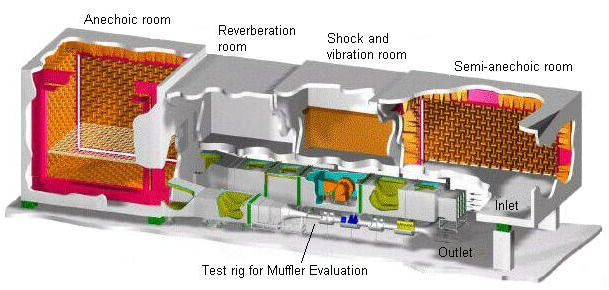
\includegraphics[scale=0.6]{MWL_flow_acoustic_test_rig}
    \caption{MWL flow acoustic test rig}
\end{figure}
The laboratory is equipped with a huge fan. For our experiments, this fan was link to the anechoic room. The pressure increases and a flow was created in a rectangular rig. The anechoic room reduces the sound produced by the fan into the rig. This fan was controlled by a computer. During my master thesis, we had to fix the cooling system to be able to run the fan at 100\% of its capacity. 
\begin{figure}[H] \centering
    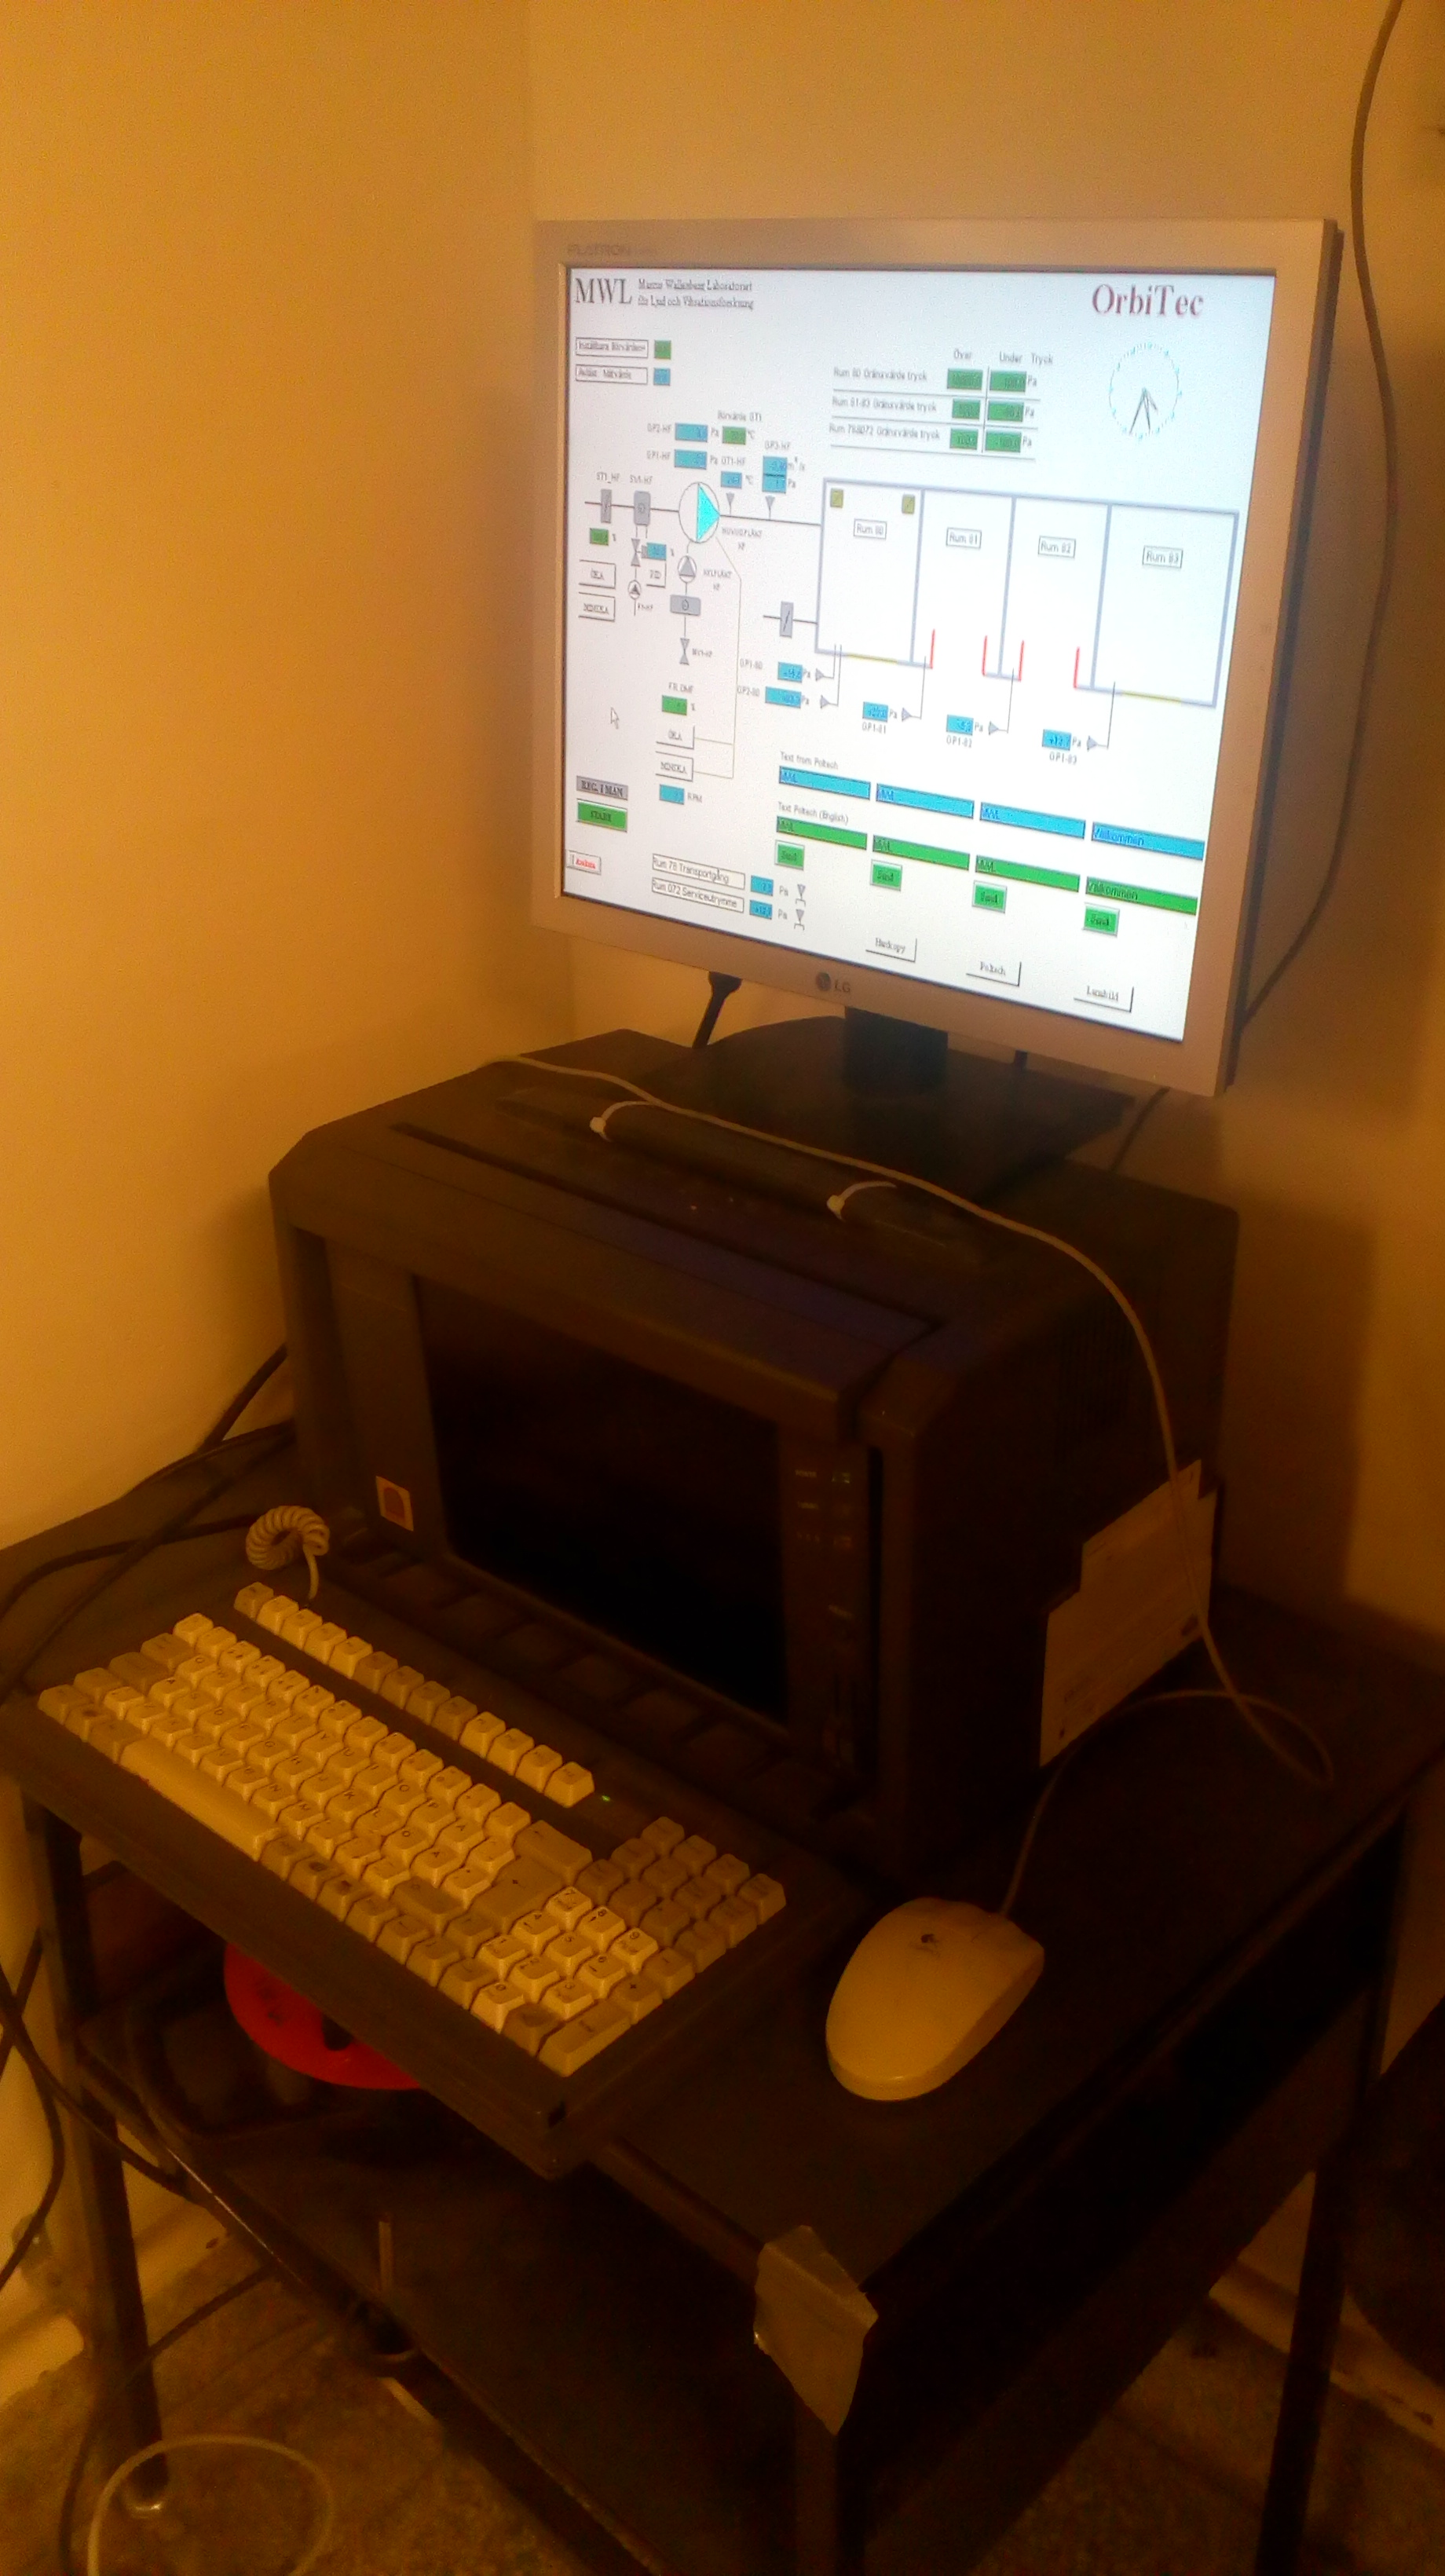
\includegraphics[scale=0.05]{ExpSetup3}
    \caption{Picture of the fan software}
\end{figure}\clearpage
%------------------------------------------------------------------------------------------------------------
%------------------------------------------------------------------------------------------------------------
\subsubsection{The rig setup}
The setup is divided in three parts: 
\begin{itemize}
    \item Upstream numbered 1
    \item Lined section numbered 2
    \item Downstream numbered 3
\end{itemize}
\begin{figure}[H] \centering
    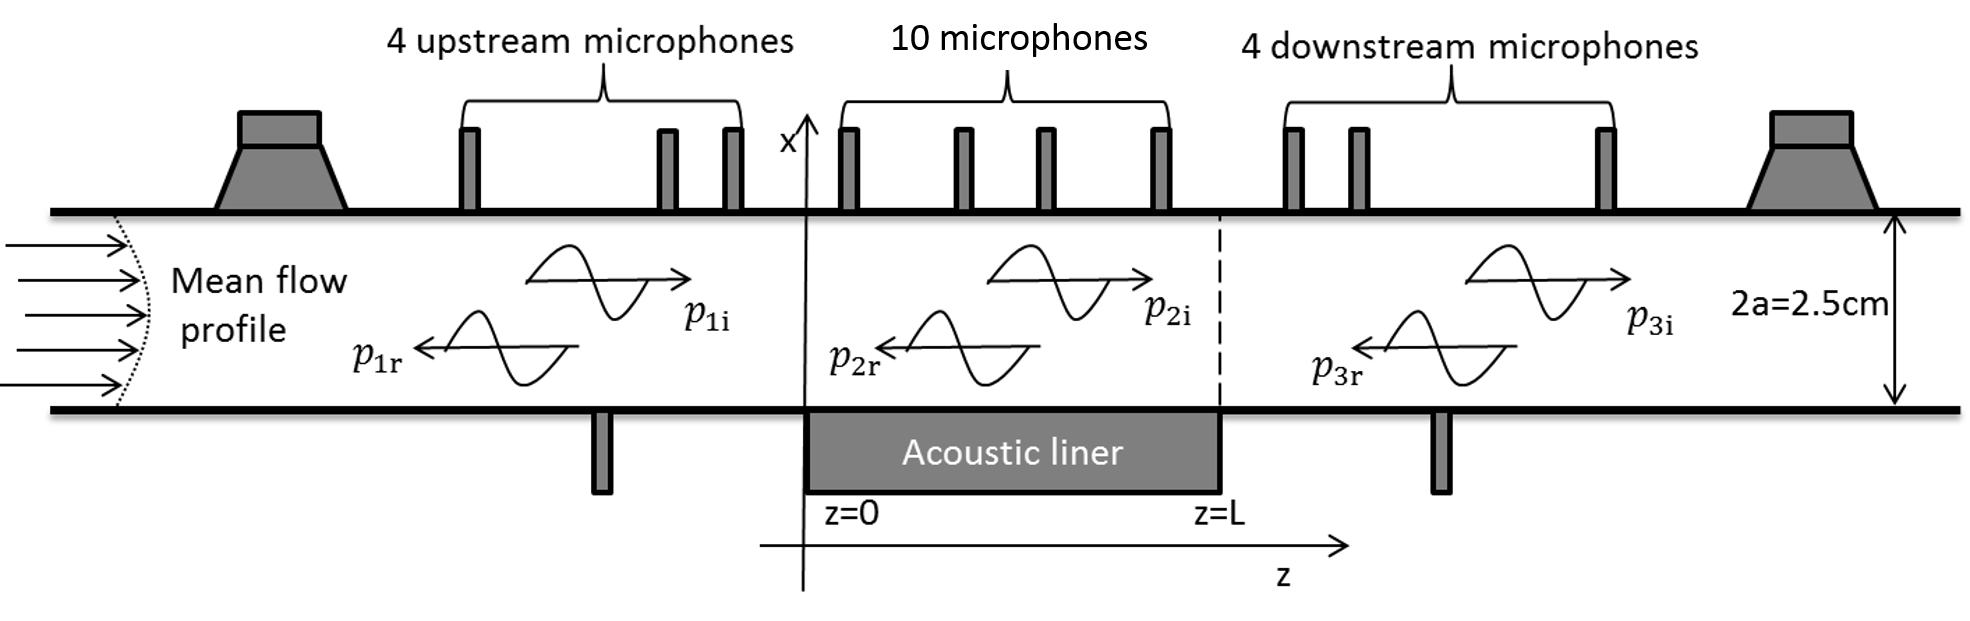
\includegraphics[scale=0.4]{Sketch_KTH_rig}
    \caption{Sketch of liner test setup at KTH}
\end{figure}
2 loudspeakers and 16 microphones were used:
\begin{itemize}
    \item 6 microphones to do the wave decomposition (3 at each upstream and downstream sides). Note than that 4 microphones were supposed to be used at the beginning.
    \item 10 microphones in the lined sections to measure the pressure field.
\end{itemize}
The termination of the rig is composed by a muffler. The reflection was very low but not equal to zero at the end of the rig.
\begin{figure}[H] \centering
    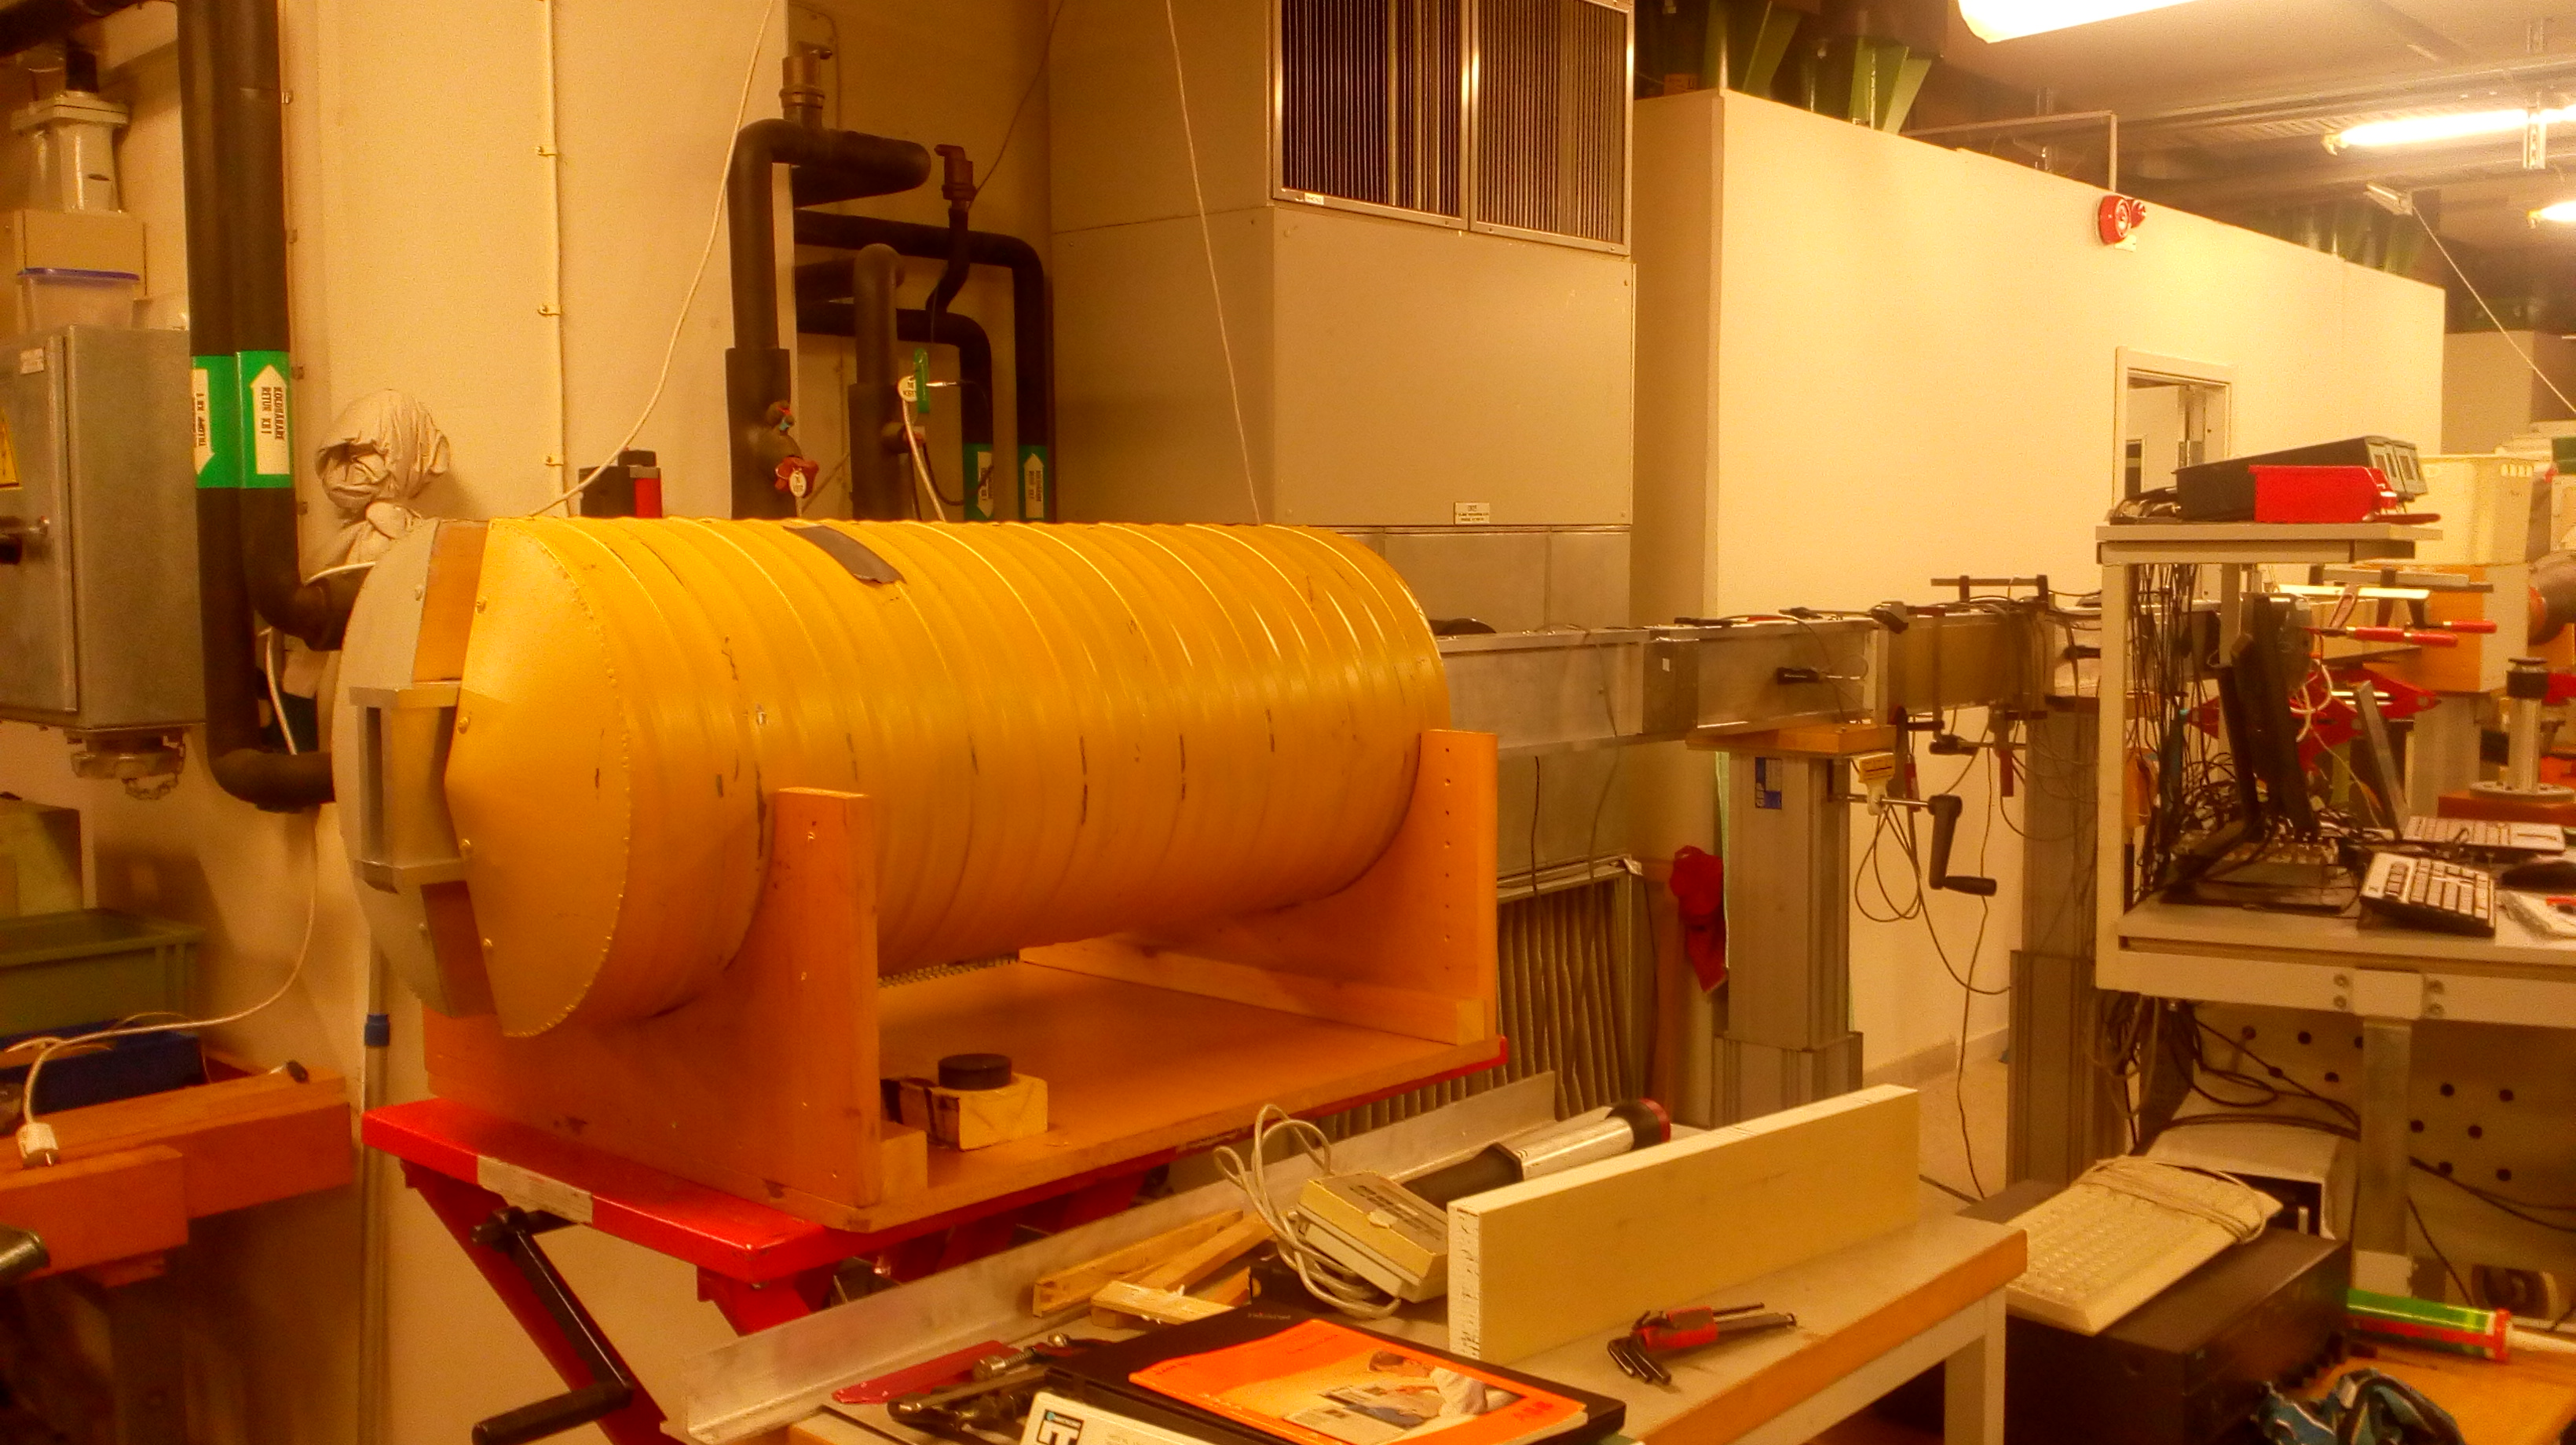
\includegraphics[scale=0.1]{ExpSetup1}
    \caption{Picture of the Rig and the anechoic termination}
\end{figure}
\begin{figure}[H] \centering
    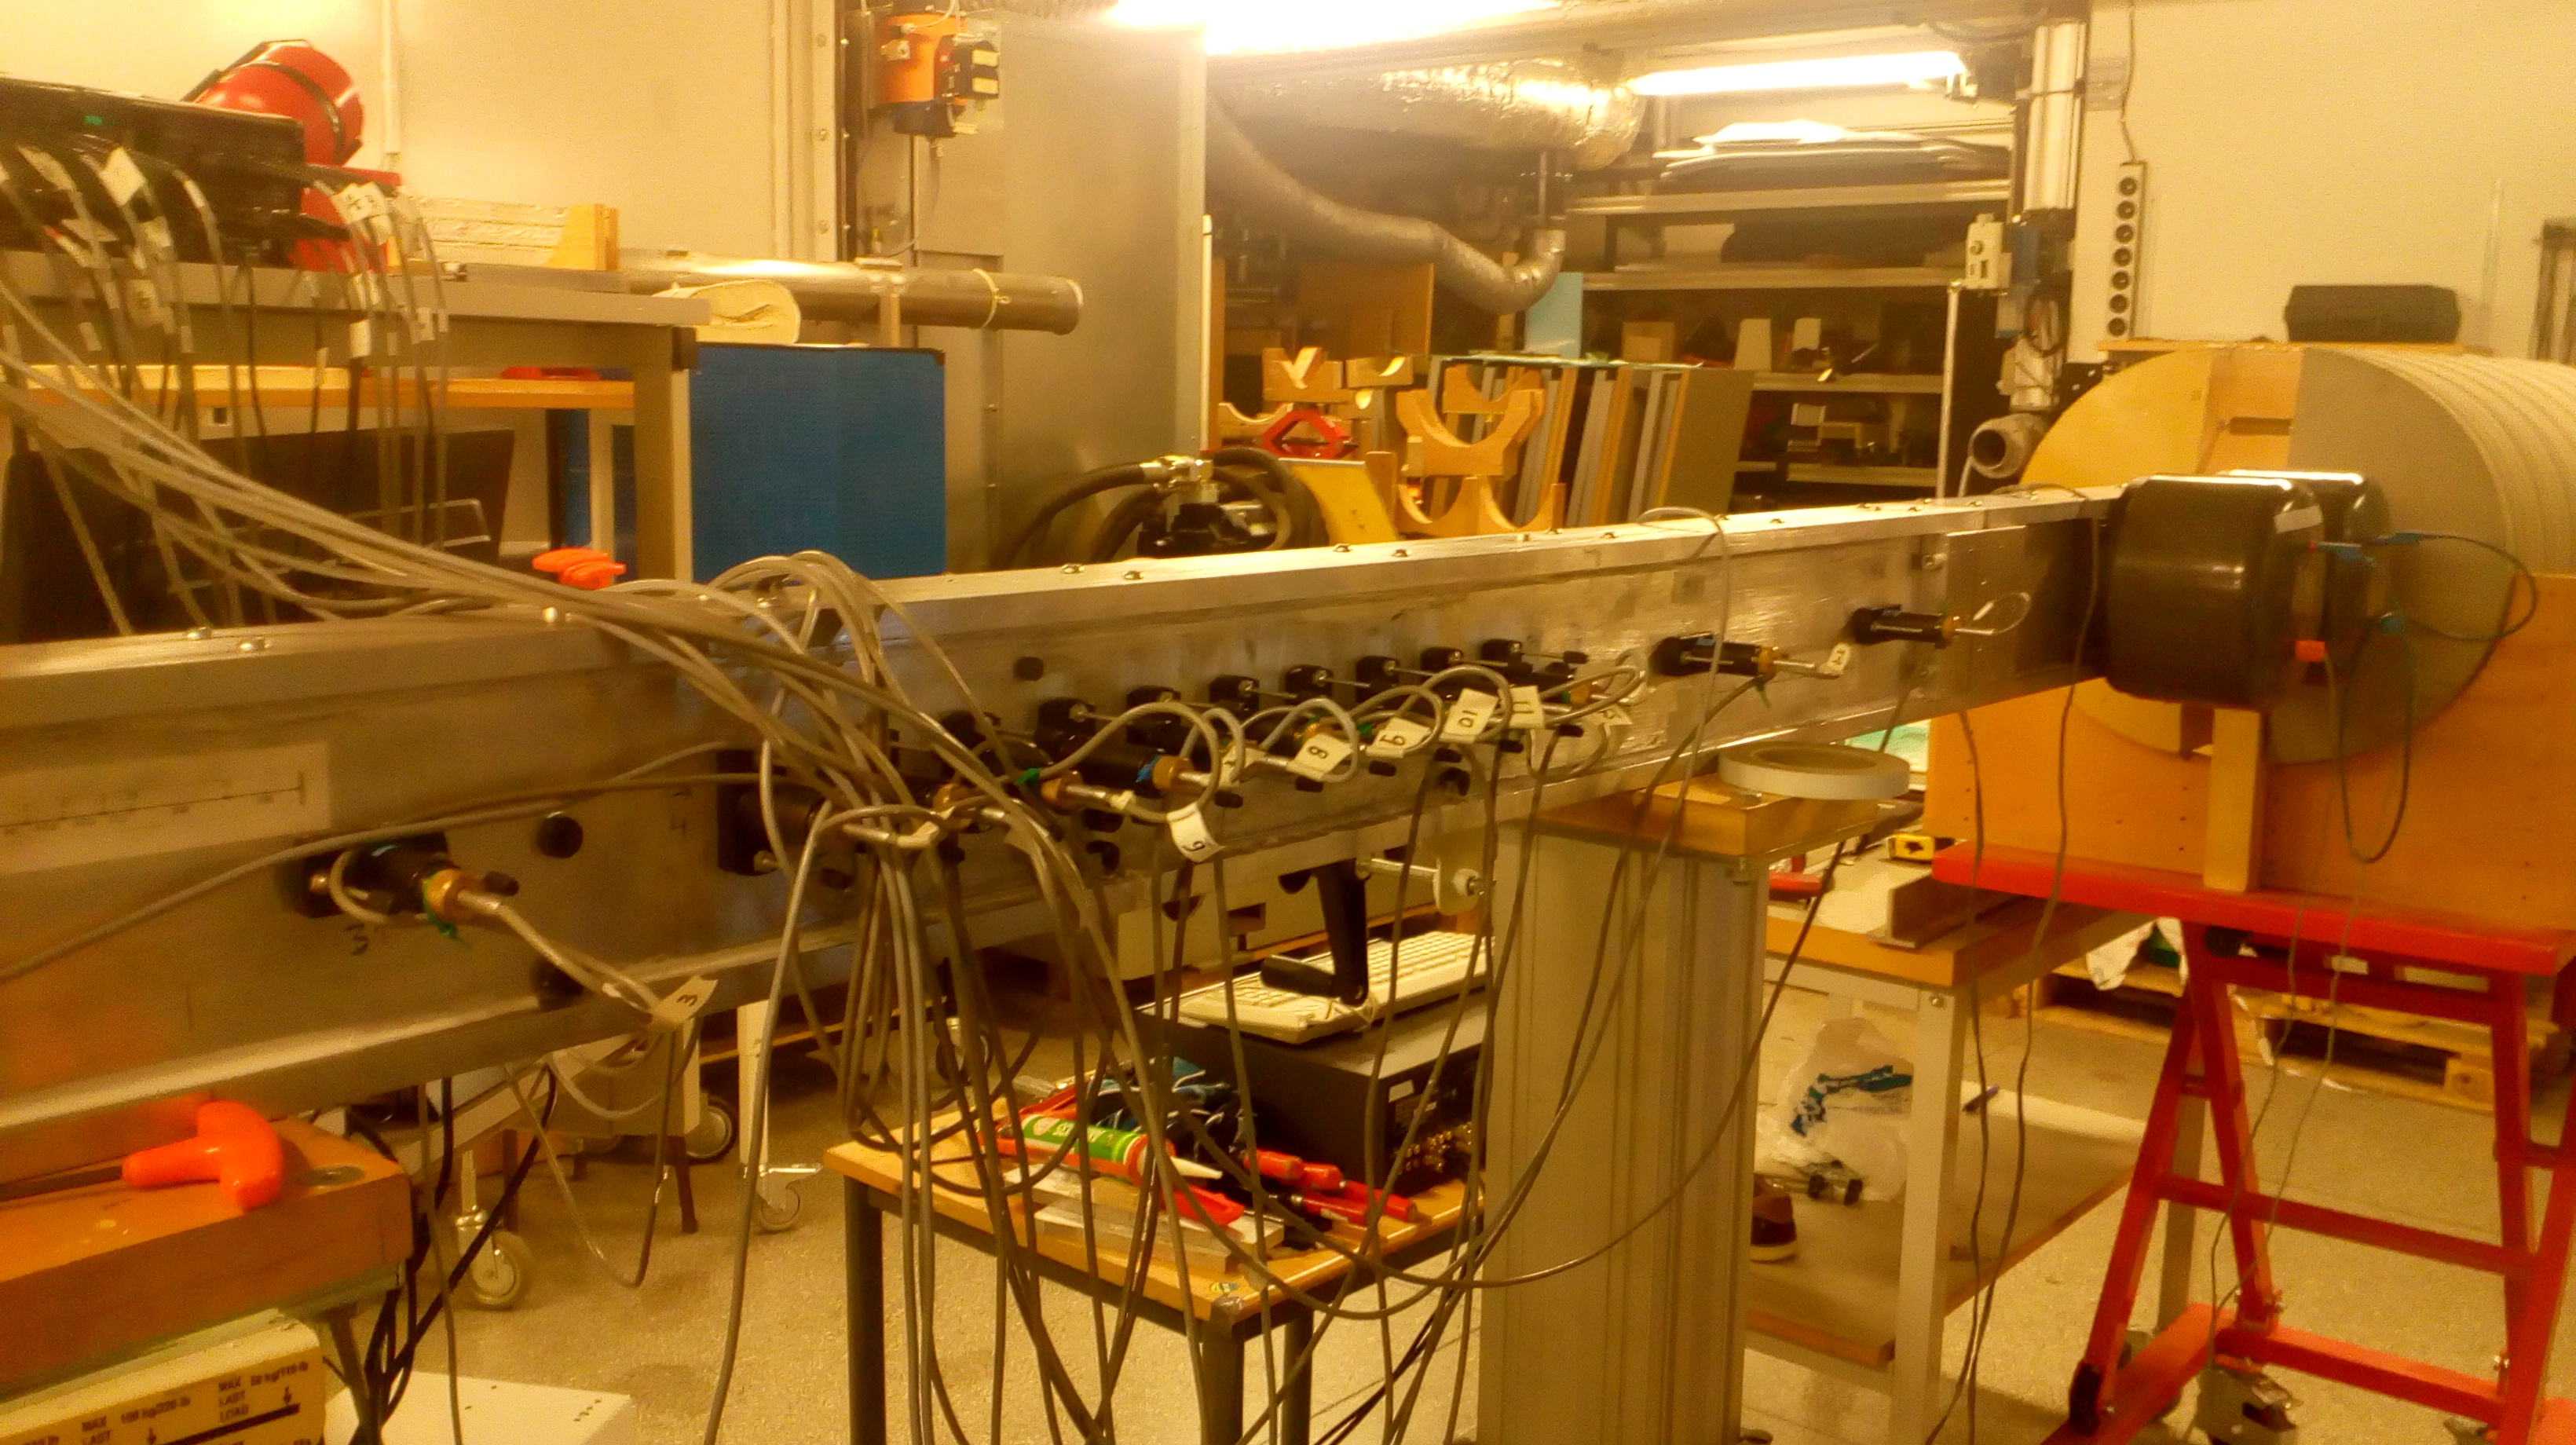
\includegraphics[scale=0.1]{ExpSetup2}
    \caption{Picture of the 16 microphones and the downstream loudspeaker}
\end{figure}
\noindent The liner is fixed flush with the wall. Any leakage can change the acoustic field.
\begin{figure}[H] \centering
    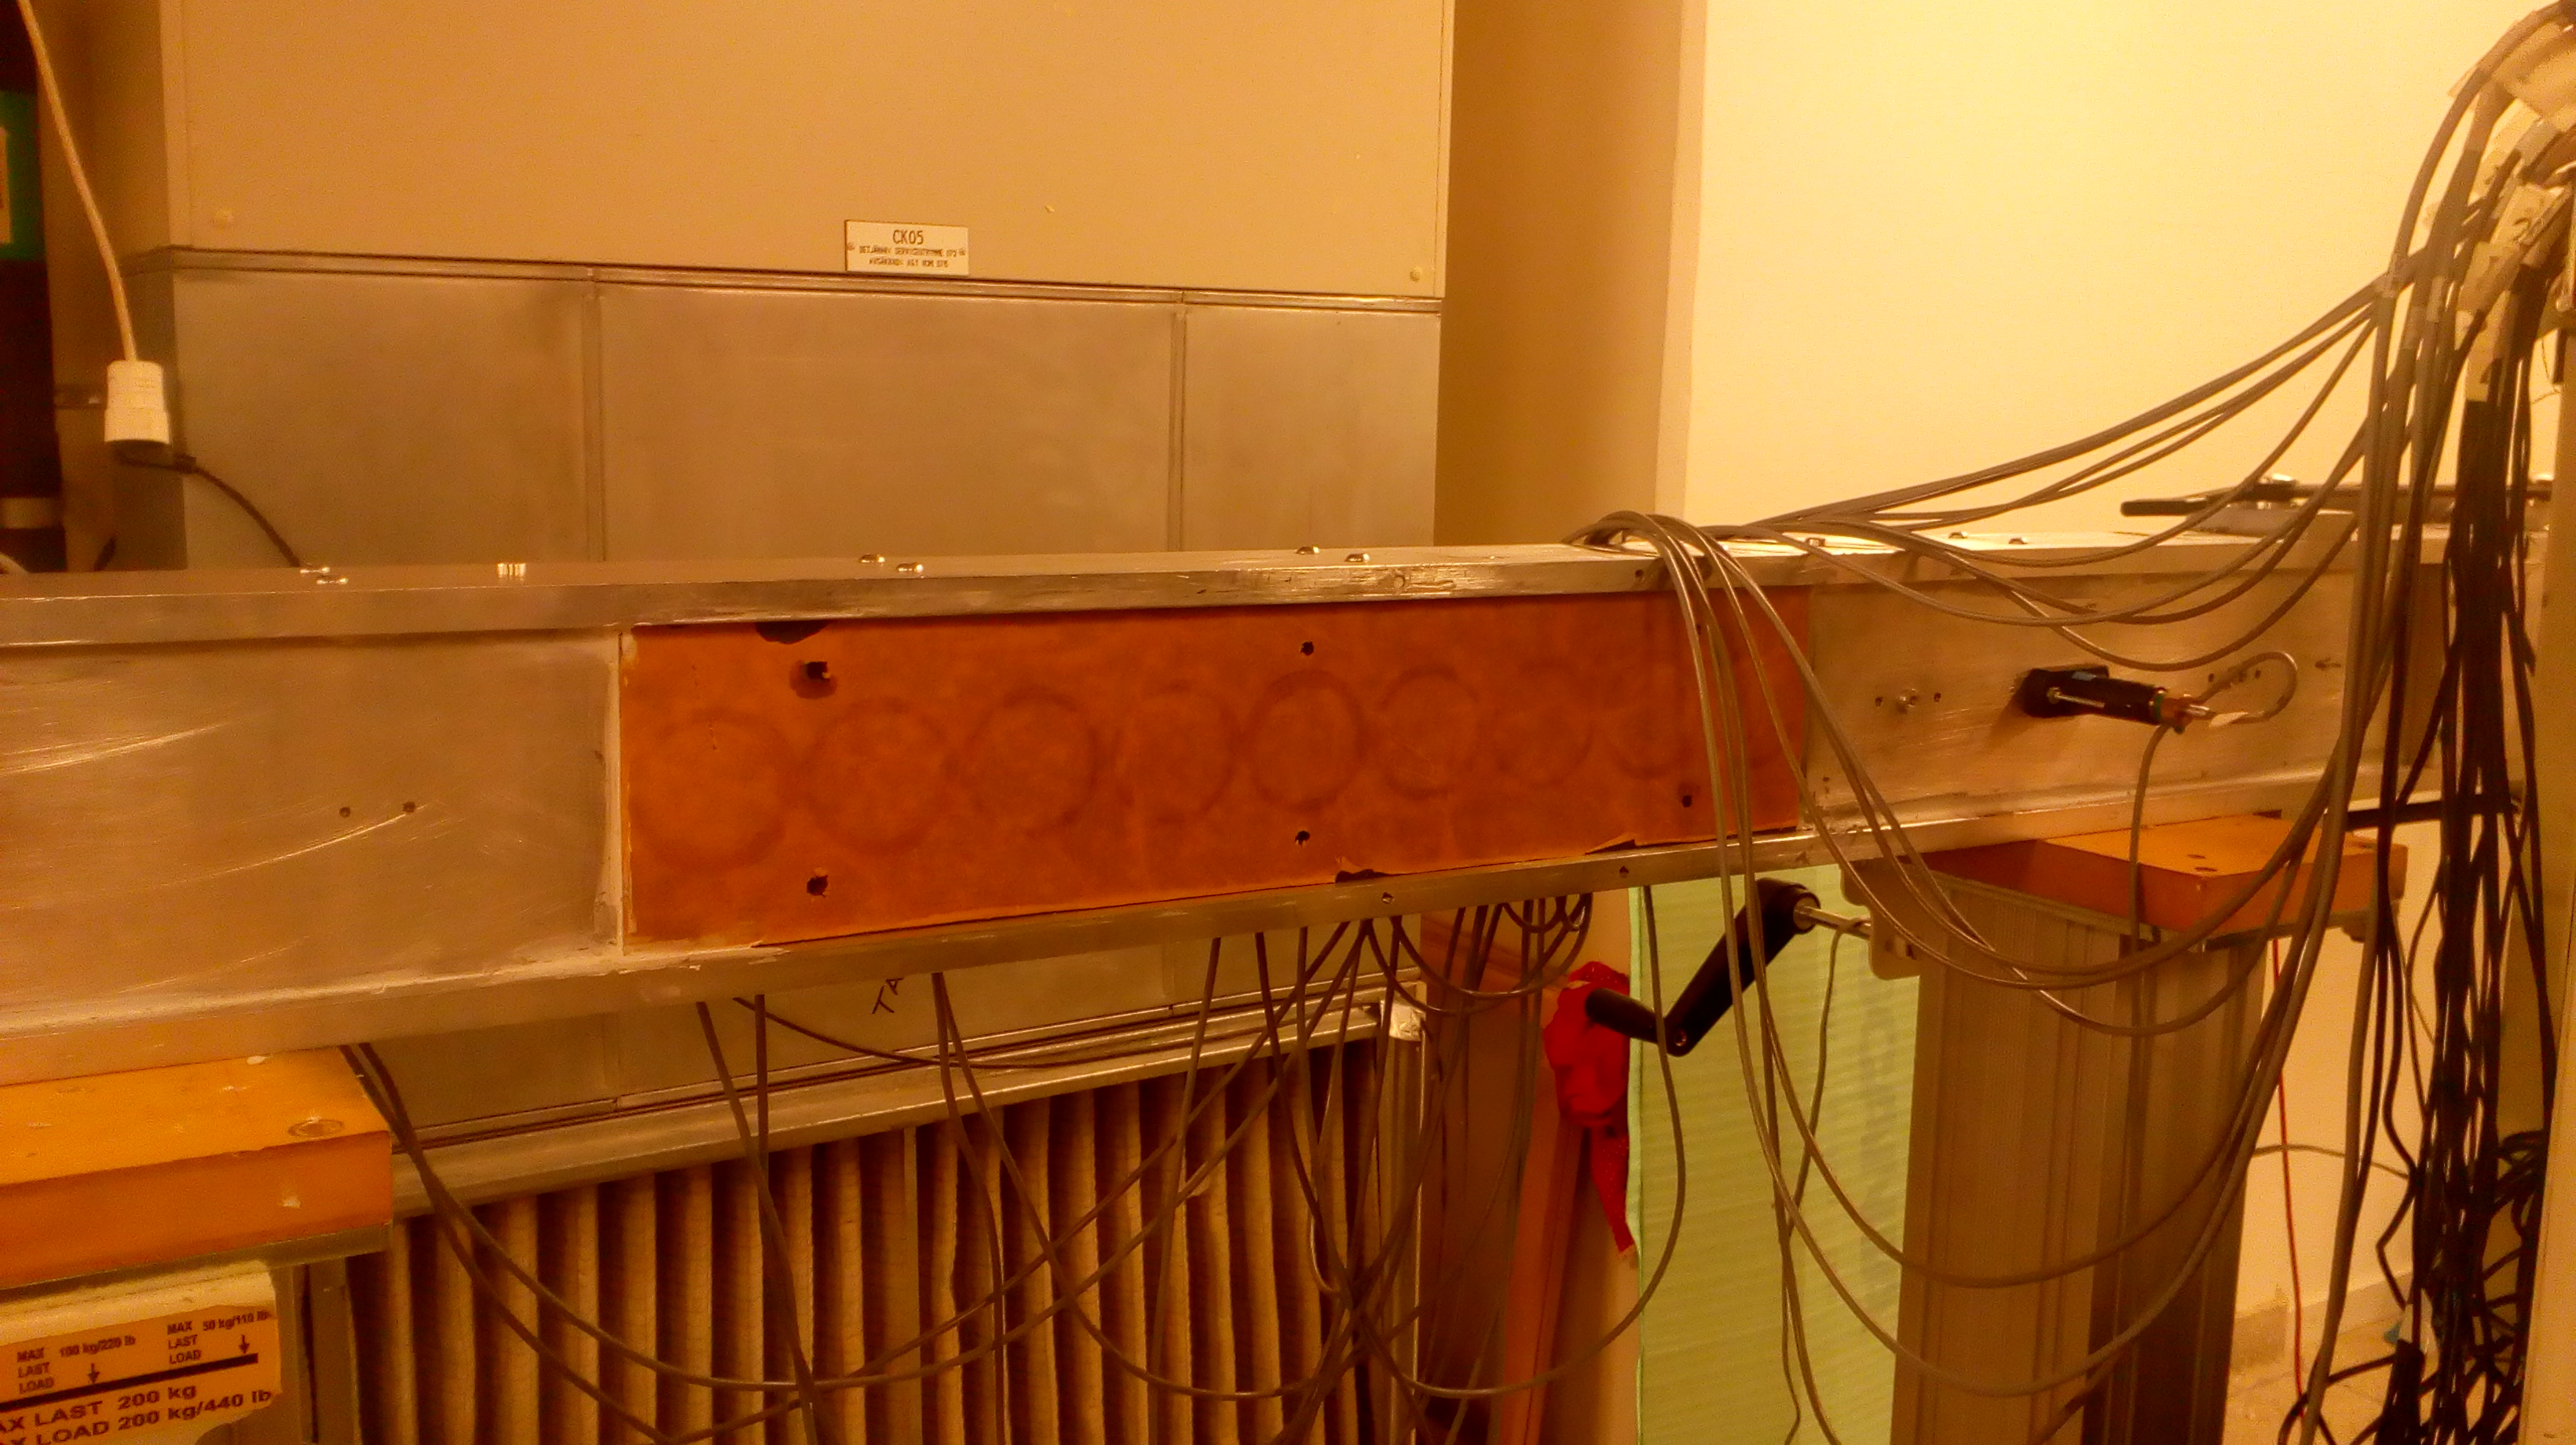
\includegraphics[scale=0.08]{ExpSetup5}
    \caption{Picture of the acoustic liner fixed in the rig}
\end{figure}
\noindent The velocity of the flow has to be measured. The \nameref{sec:AppendixC} describes how to get the mean flow in the duct with the Pitot tube.
\begin{figure}[H] \centering
    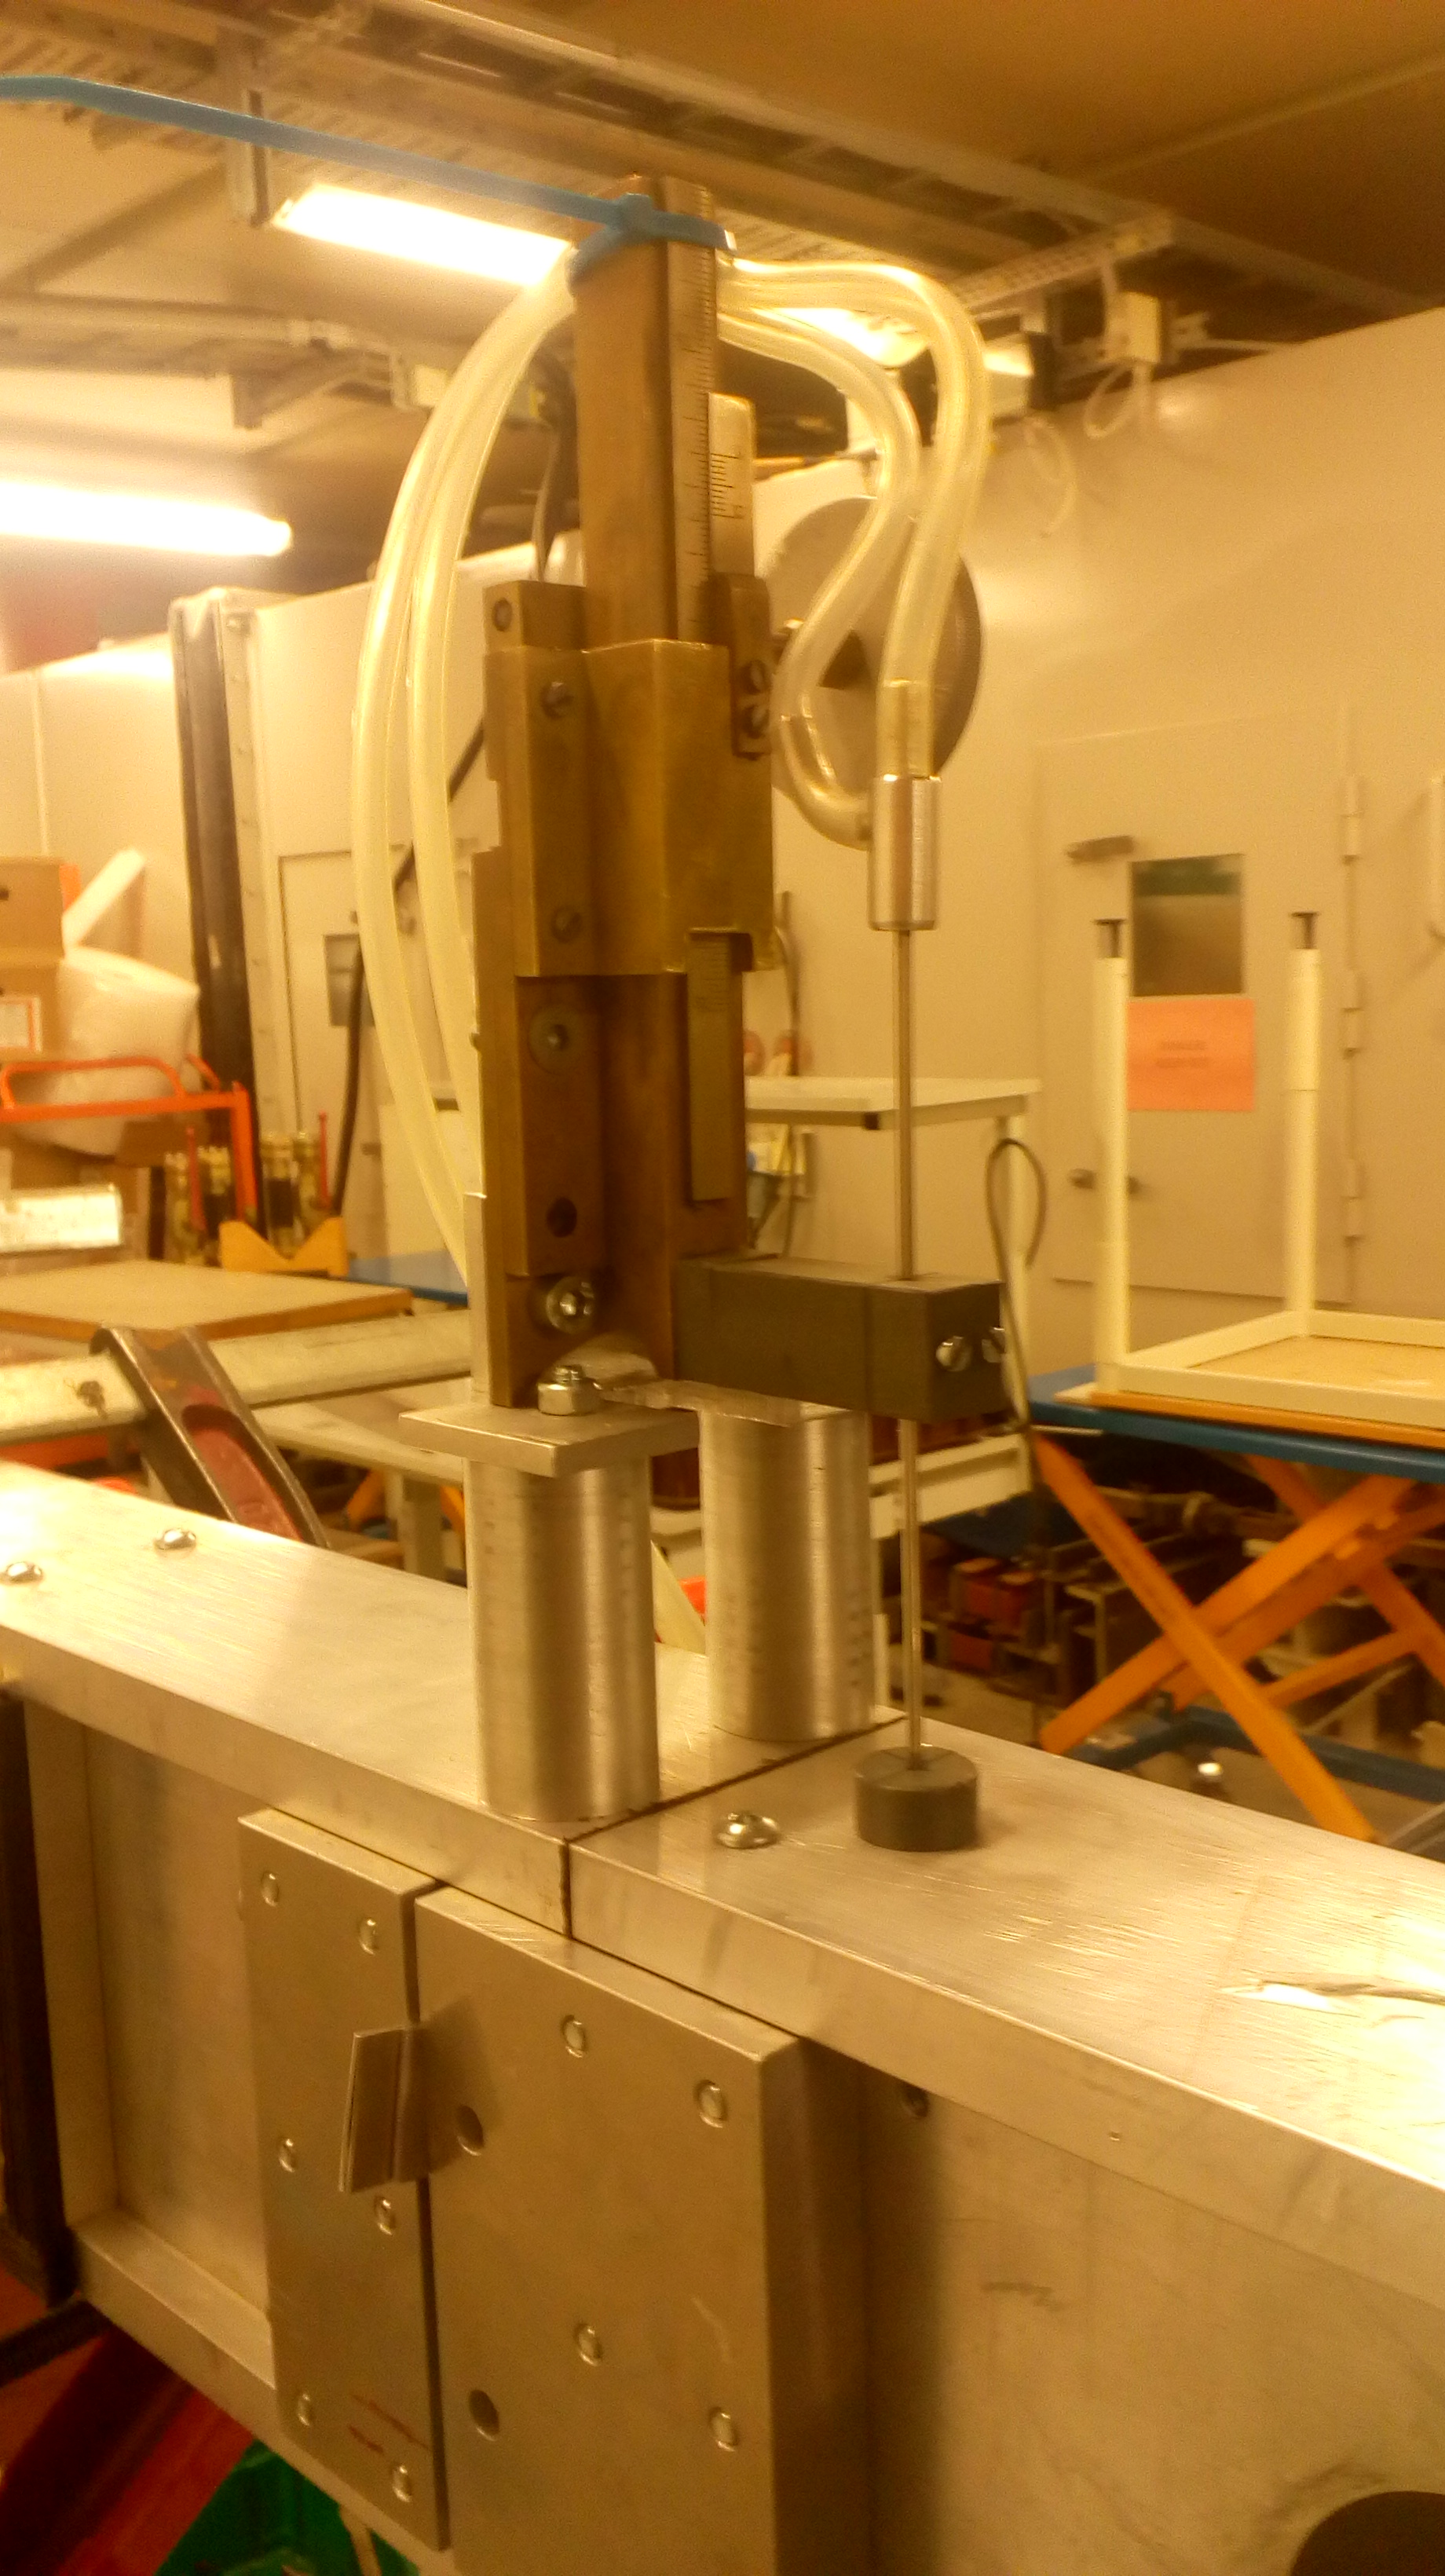
\includegraphics[scale=0.05]{ExpSetup4}
    \caption{Picture of the Pitot tube}
\end{figure}
%------------------------------------------------------------------------------------------------------------
%------------------------------------------------------------------------------------------------------------
\subsubsection{Acquisition chain}
\begin{figure}[H] \centering
    \begin{subfigure}{.5\textwidth}\centering
     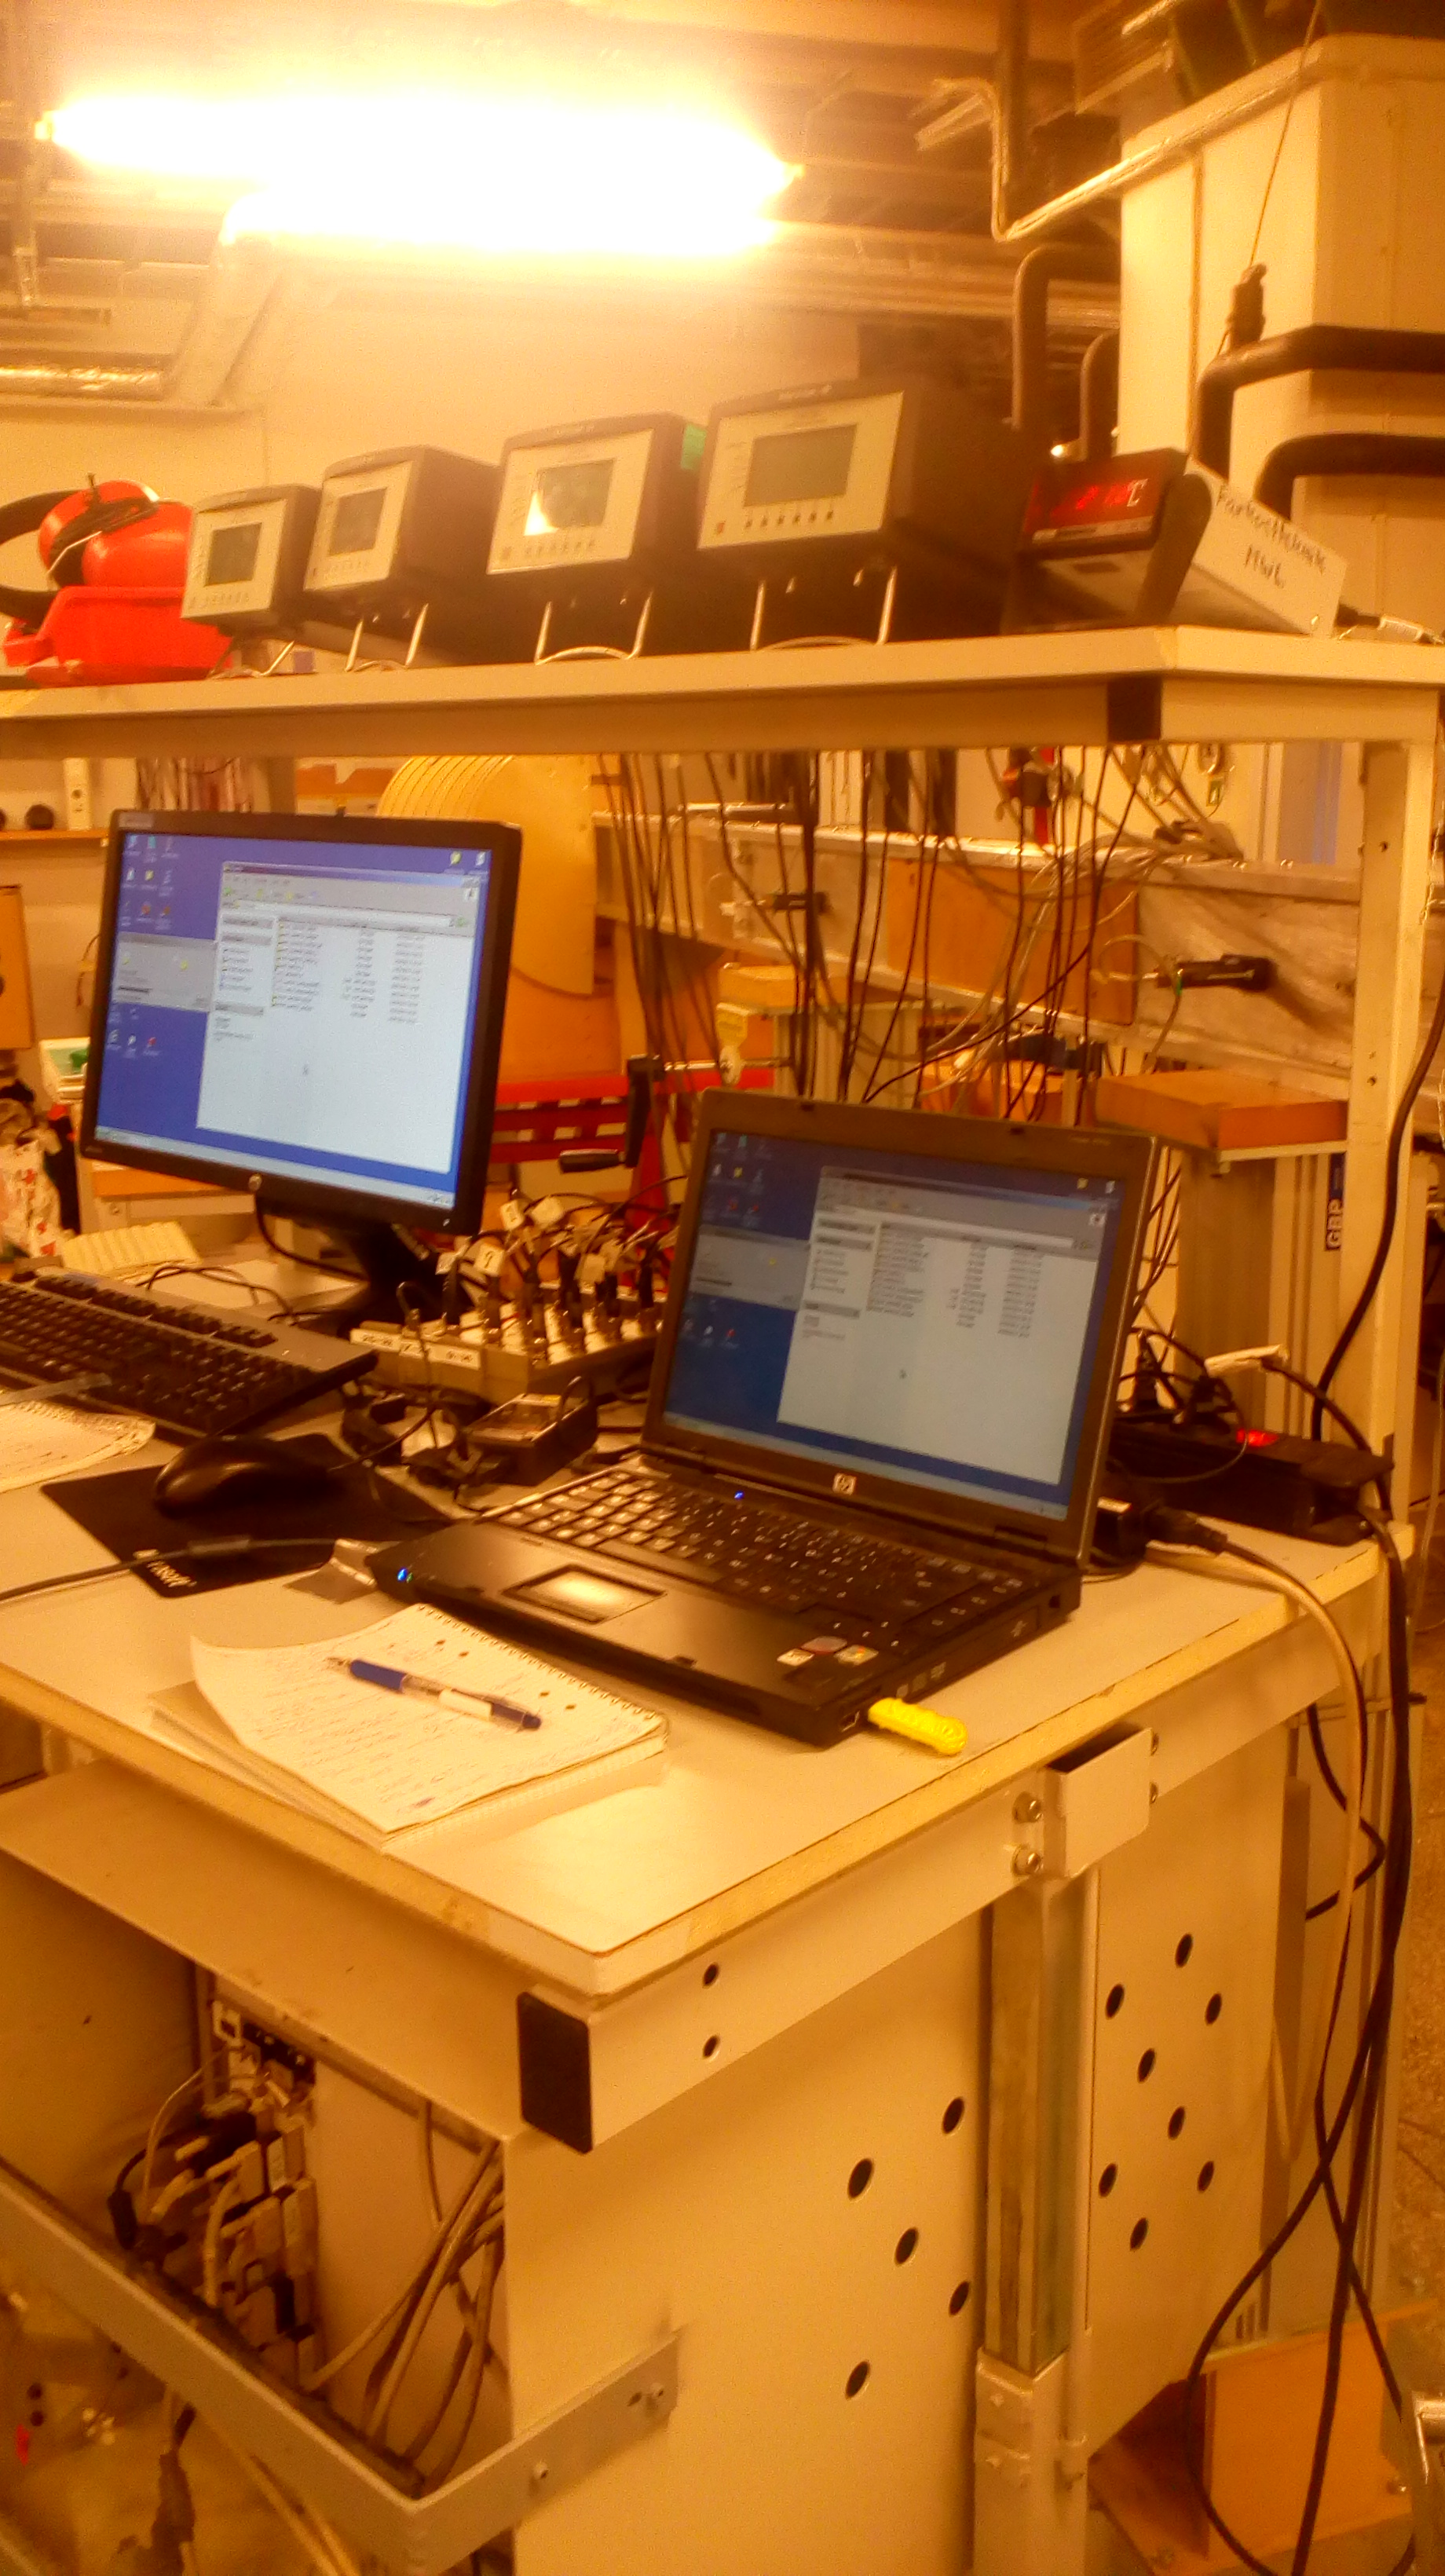
\includegraphics[width=.8\linewidth]{Acquisition1}
     \caption{Picture computer and nexuses}
    \end{subfigure}%
    \begin{subfigure}{.5\textwidth}\centering
     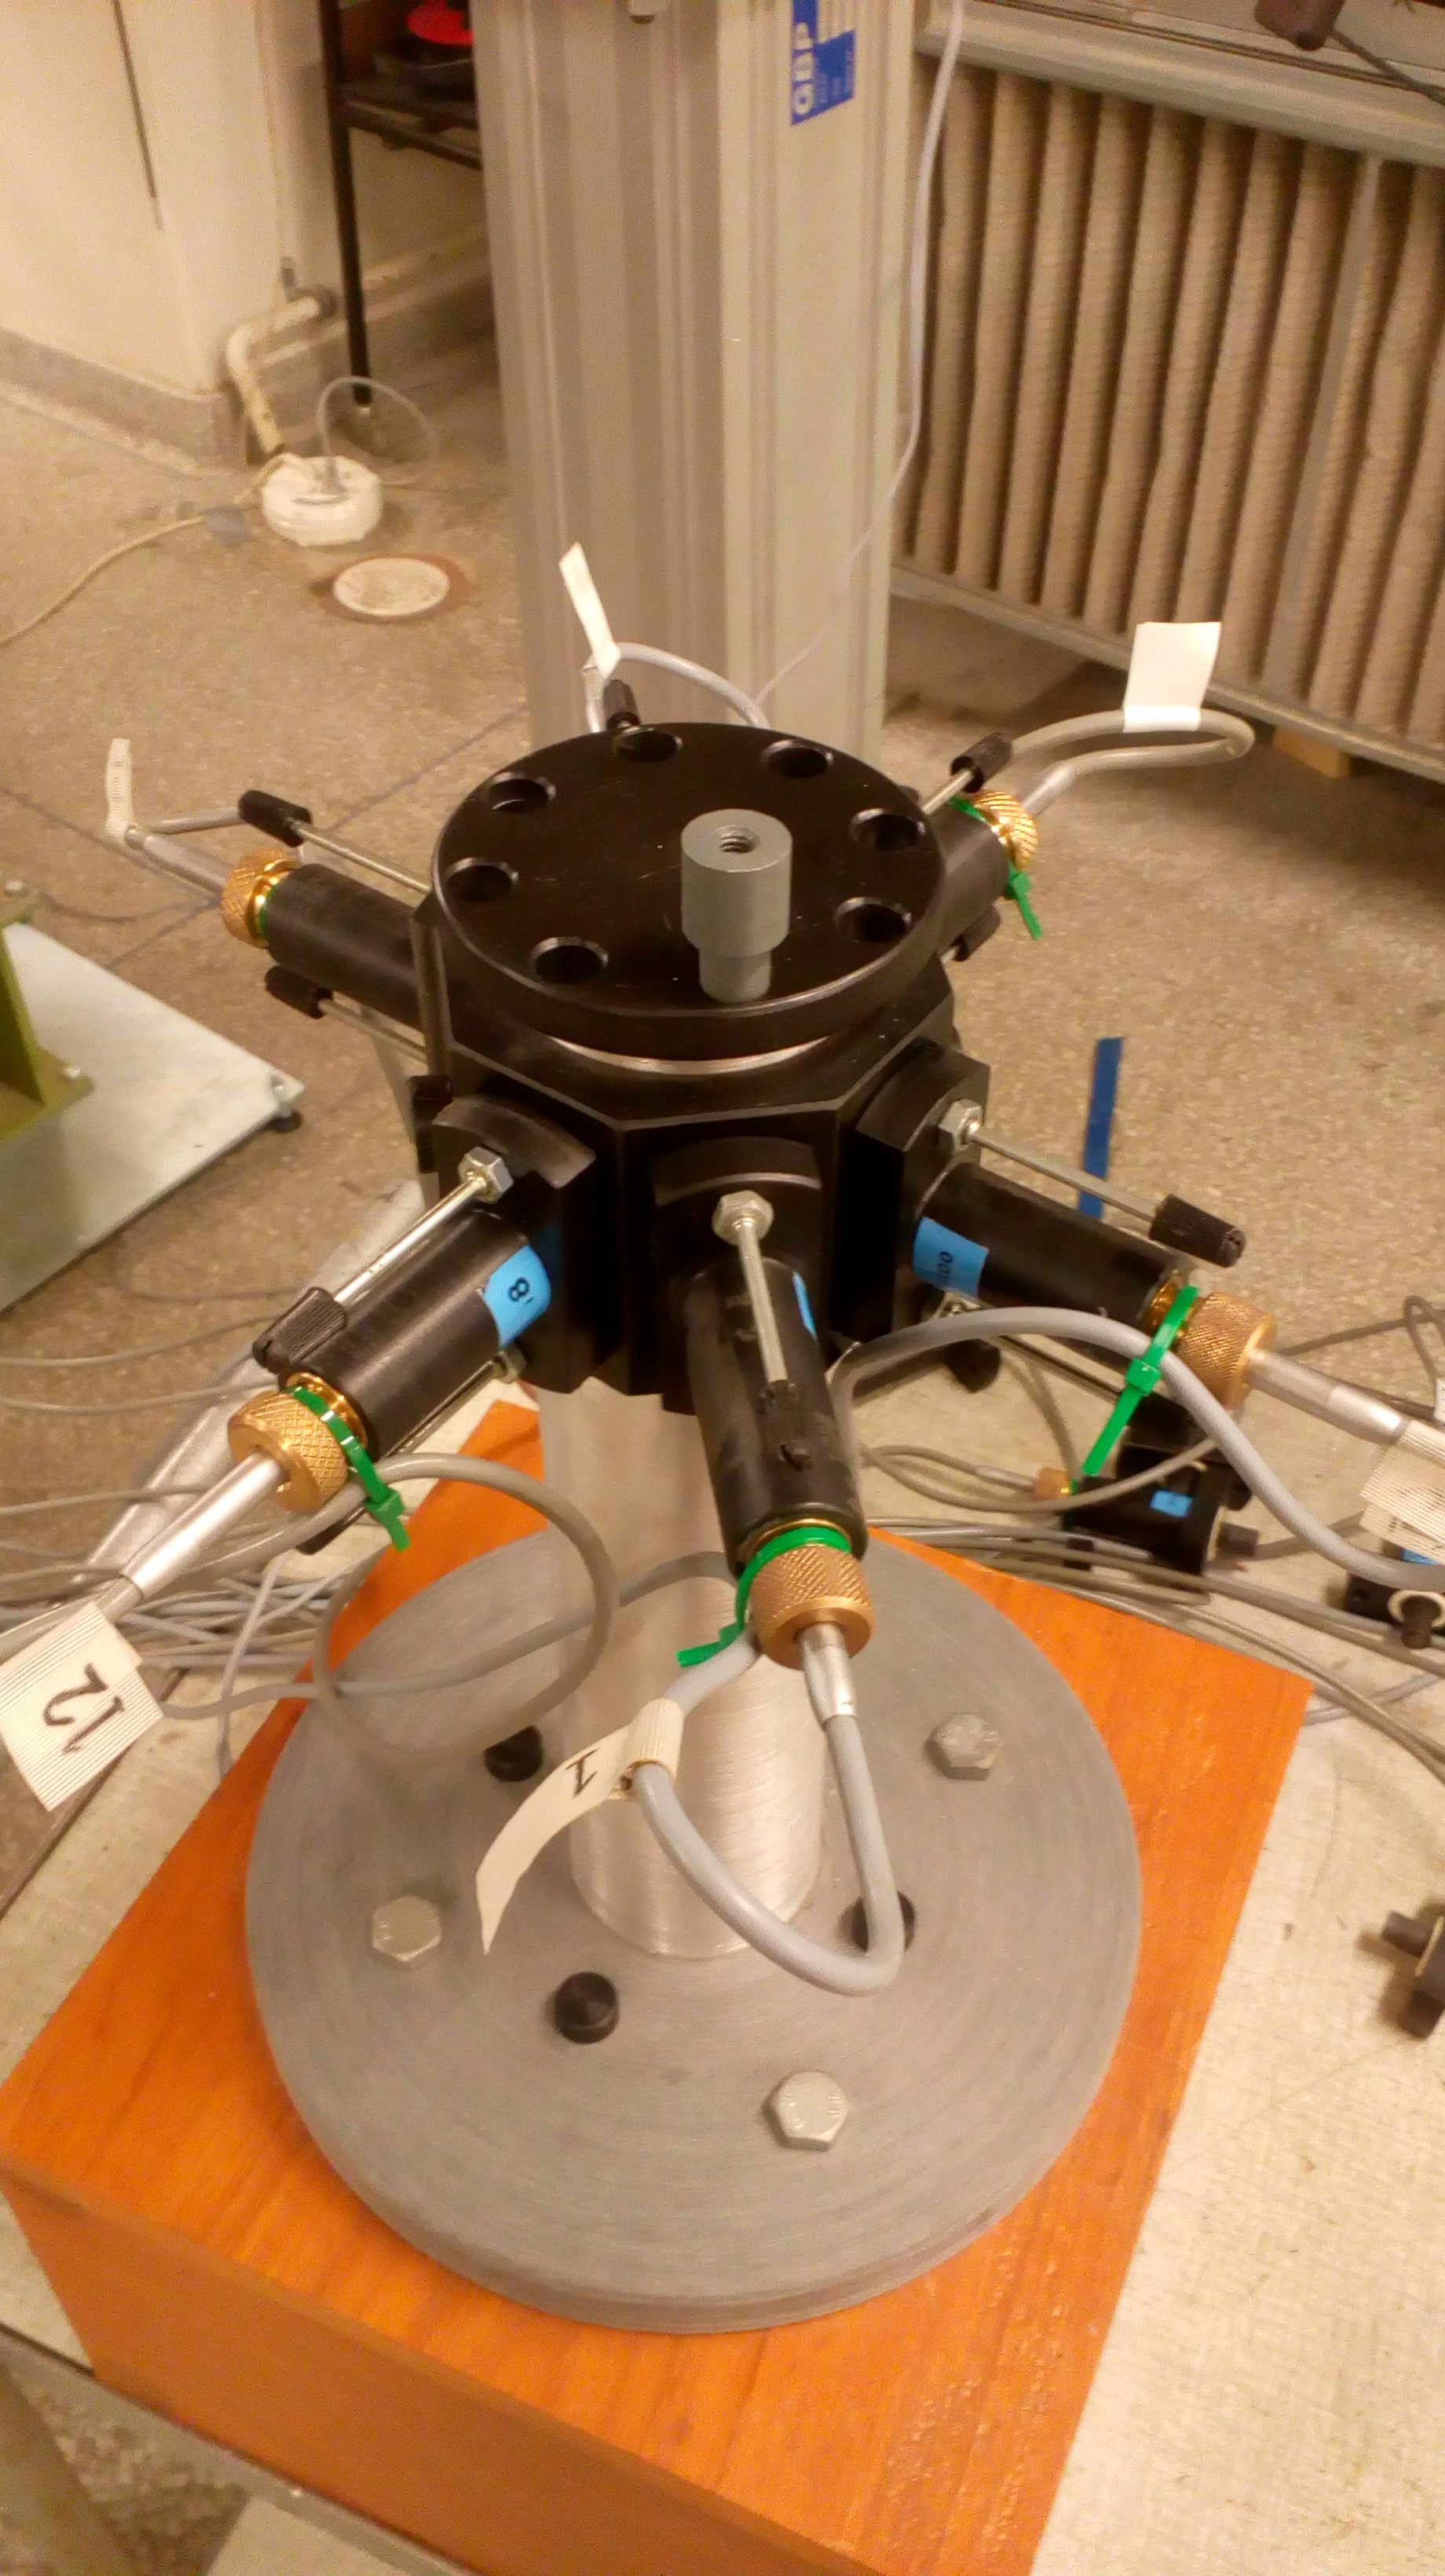
\includegraphics[width=.8\linewidth]{Acquisition2}  
      \caption{Picture of the  calibration tube}
    \end{subfigure}
    \caption{Pictures of experimental devices}
\end{figure}
\noindent A HP-VXI system creates an sinus excitation signal. This sinal is amplified by a classic amplifier and the loudspeaker transforms the signal into an acoustic sinus wave. The Brüel and Kjaer microphones provide an electric signal which is treat by a Nexus device. To get the true pressure value, the sensitivity and the gain of the nexus have to be saved. The HP-VXI system does also the acquisition. A Matlab program saves the temporal data into a file.\\
This code provides by Luck \cite{Luck_thesis} has also other options to improve the quality of the measure:
\begin{itemize}
    \item The excitation is calibrated before the measure to respect a positive plane wave $p^+$ equal to $1Pa$. This calibration should avoid any non-linear pressure effect (this option is more important for high excitation level)
    \item The time of the acquisition depends of the variance of the measured signals. The accuracy of the data increases with the measured time. But the temperature into the rig increases slowly during the measurement. The measure has to relatively fast to avoid any temperature effect.
    \item By the same idea, the frequencies studied are randomized. The effect of the temperature variation are distributed, and any temperature trend appears.
\end{itemize}
To get a more accuracy measure, the microphones are calibrated before. A stationary wave is created in a tube. The axial position of the microphones are strictly the same as are the measured pressures. The transfer functions are calculated, the reference is the first microphone.
%------------------------------------------------------------------------------------------------------------
\subsubsection{Frequency domain and scattering matrix}
The measures are time dependant: 
\begin{figure}[H] \centering
    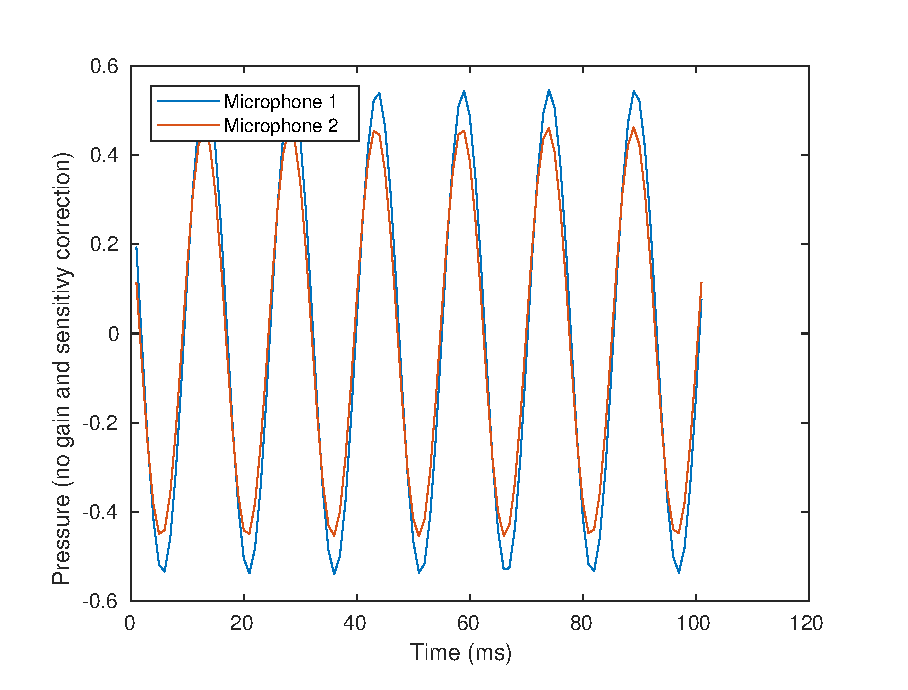
\includegraphics[scale=0.7]{PTimeNoLiner}
    \caption{Time dependant signal}
\end{figure}
The Hilbert transform is used to get the estimated transfer function:
\begin{figure}[H] \centering
    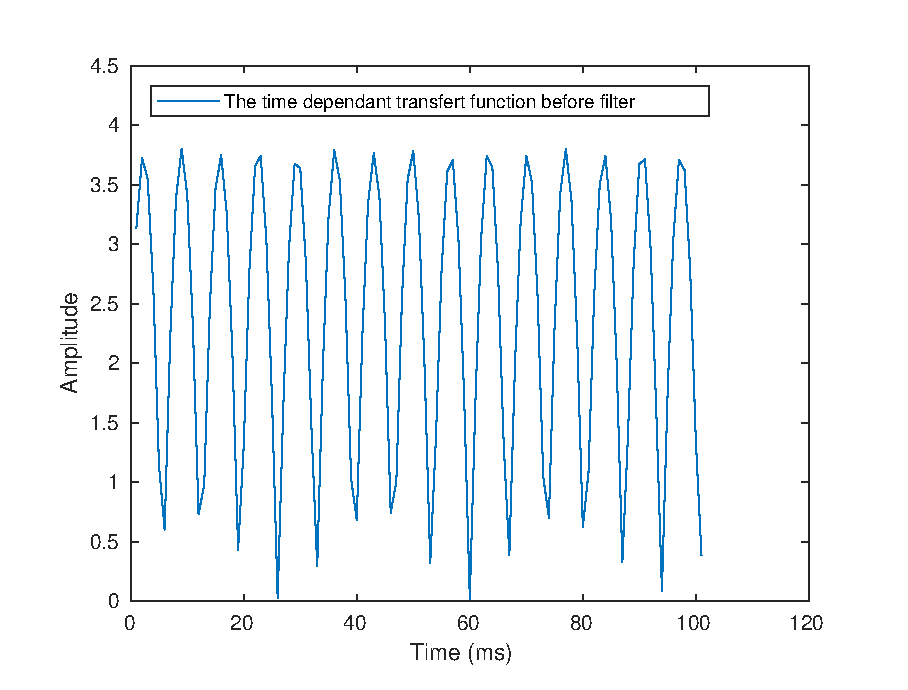
\includegraphics[scale=0.7]{PHilbertNoLiner}
    \caption{Estimated transfer function time dependant before windows filtering}
\end{figure}
A windows is determined which contained a whole number of sinus. The signal is filtered to get the true transfer function:
\begin{figure}[H] \centering
    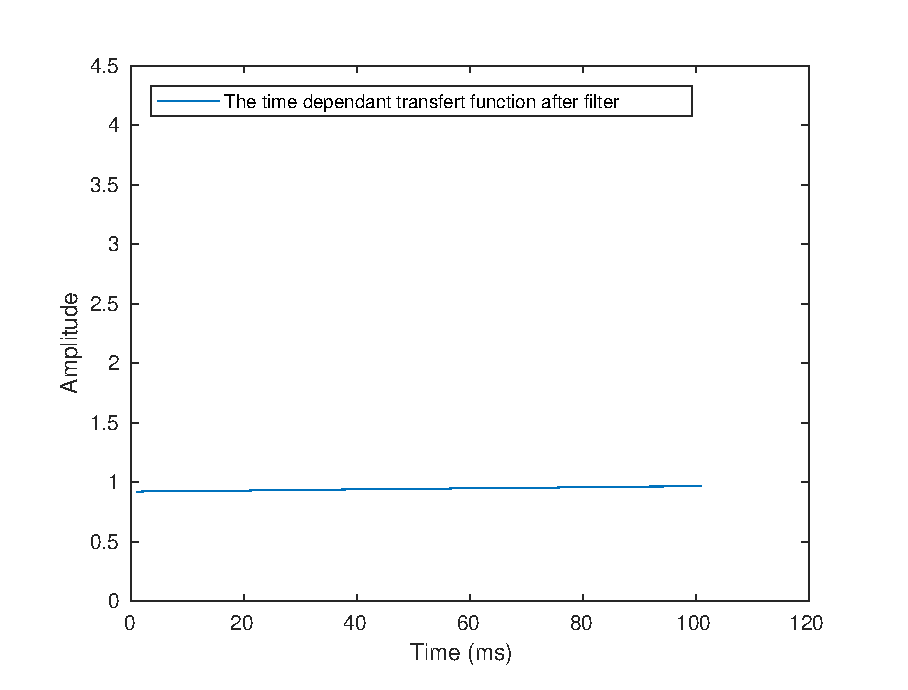
\includegraphics[scale=0.7]{PHilbertFiltreNoLiner}
    \caption{True transfer function time dependant after windows filtering}
\end{figure}
With the source reference, all the complex pressures are determined.
%------------------------------------------------------------------------------------------------------------
%------------------------------------------------------------------------------------------------------------
\subsection{Reference: hard wall case}
3 mach flows are studied: $M=0, M=0,08\ \text{and}\ M=0.16$. The frequency is between 700Hz and 1200Hz.\\
It's very difficult to get accurate measures in a rig. The mean flow adds lot of in-stationary noise. In a way to gain confidence in the results, a measure of the hard wall duct are performed. The problem is reduce to an infinite hard duct. Only a plane wave propagates because the higher modes are over the cut-off frequency. In this simple case the two transmission coefficients should be 1 and the reflecxion coefficients equal to zero.\\
The scattering matrix measured:
\begin{figure}[H] \centering
    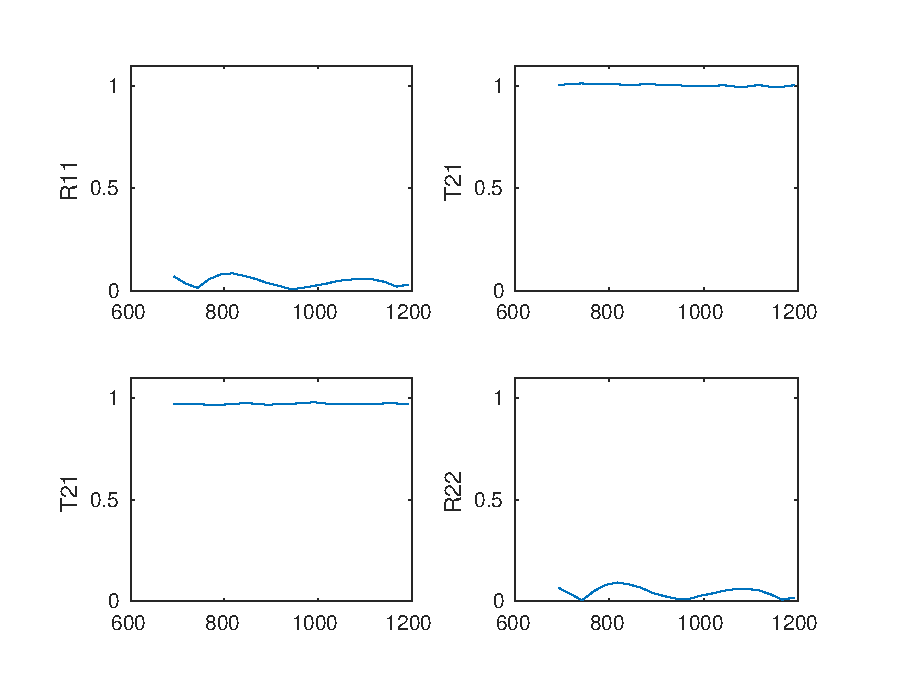
\includegraphics[scale=0.7]{ScatNoLin}
    \caption{Scattering matrix: Hard wall and no flow }
\end{figure}
\noindent The transmission coefficients are very close to 1. The reflection is a little bit higher than expected. With flow, the scattering matrix stay very accurate:
\begin{figure}[H] \centering
    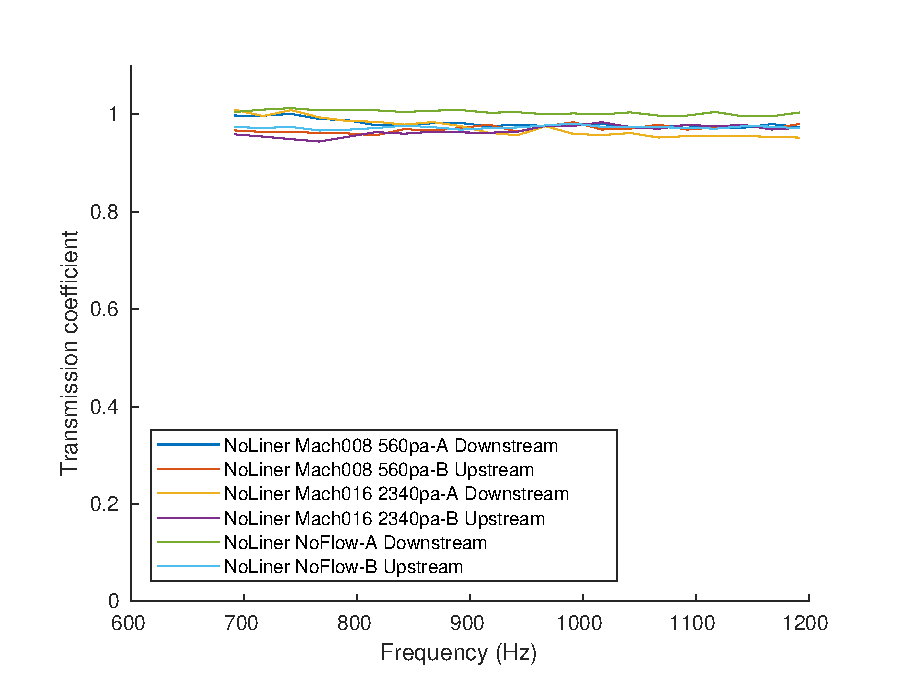
\includegraphics[scale=0.7]{TNoLinAll}
    \caption{Transmission coefficients (T21 correspond to upstream and  T12 correspond to downstream excitation): Hard wall; M=0, M=0.08, M=0.16 }
\end{figure}
%------------------------------------------------------------------------------------------------------------
%------------------------------------------------------------------------------------------------------------
%------------------------------------------------------------------------------------------------------------
%------------------------------------------------------------------------------------------------------------
\subsection{Acoustic liner}
%------------------------------------------------------------------------------------------------------------
%------------------------------------------------------------------------------------------------------------
\subsubsection{Scattering matrix and transmission loss}
\begin{figure}[H] \centering
    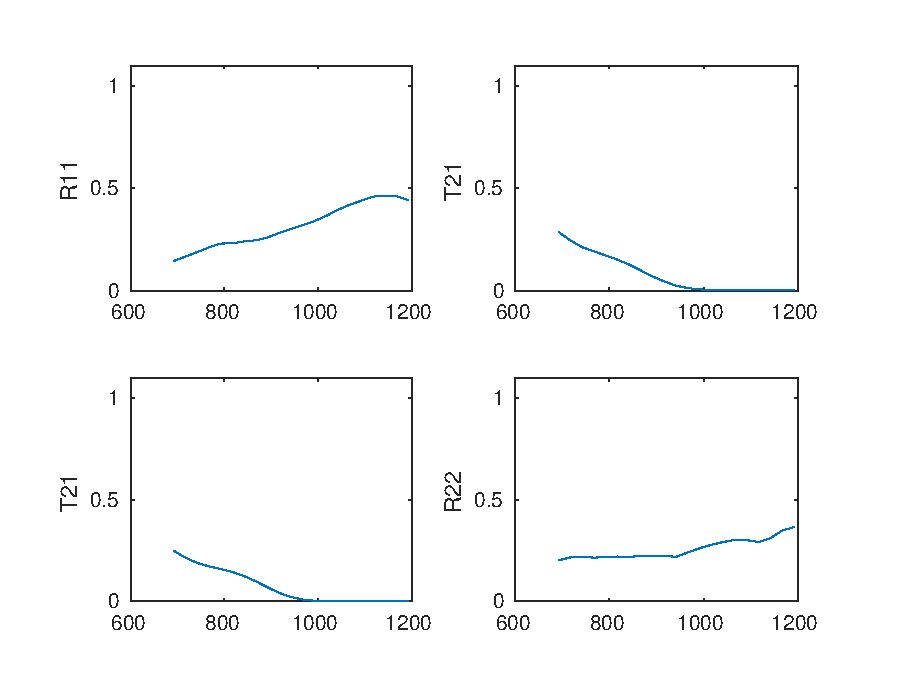
\includegraphics[scale=0.7]{ScatLinNoFlow}
    \caption{Scattering matrix: Liner and no flow}
\end{figure}
The reflection is lower than 0.5. Some energy is reflected towards the source.\\
A liner has to reduce the acoustic energy transmit to the output.
The transmission loss is directly given by the transmission coefficient:
\begin{equation}
    TL=20\text{log}(1/T)
\end{equation}
Thus, the studied parameter is the transmission coefficient. As a reminder, upstream transmission coefficient is called $T12$ and the downstream $T21$. For every case this coefficient is closed to zero, almost all the acoustic energy is absorbed or reflected.\\
These coefficients are equal for no flow. But more the velocity is high more the upstream transmission becomes higher than the downstream transmission. This effect is due to the non uniform shape flow. At the wall the acoustic wave sees an opposite velocity gradient for the upstream or downstream propagation. This effect is not taken account in the Myers boundary conditions which consider uniform flow. This difference is showed: 
\begin{figure}[H] \centering
    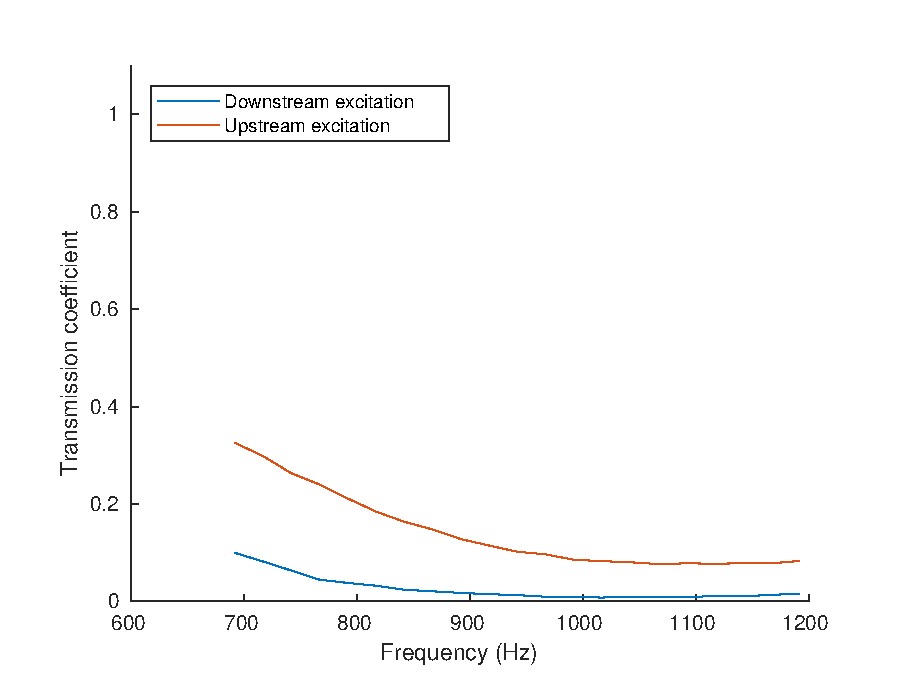
\includegraphics[scale=0.7]{TLinM016}
    \caption{Transmission coefficients: Liner 1 and M=016}
\end{figure}
Two different effects of the flow are highlighted:
\begin{itemize}
    \item Upstream excitation: the transmission increases with the mach number at low frequency
    \item downstream excitation: the efficiency of the liner increases at low frequency.
\end{itemize}
\begin{figure}[H] \centering
    \begin{subfigure}{.5\textwidth}\centering
     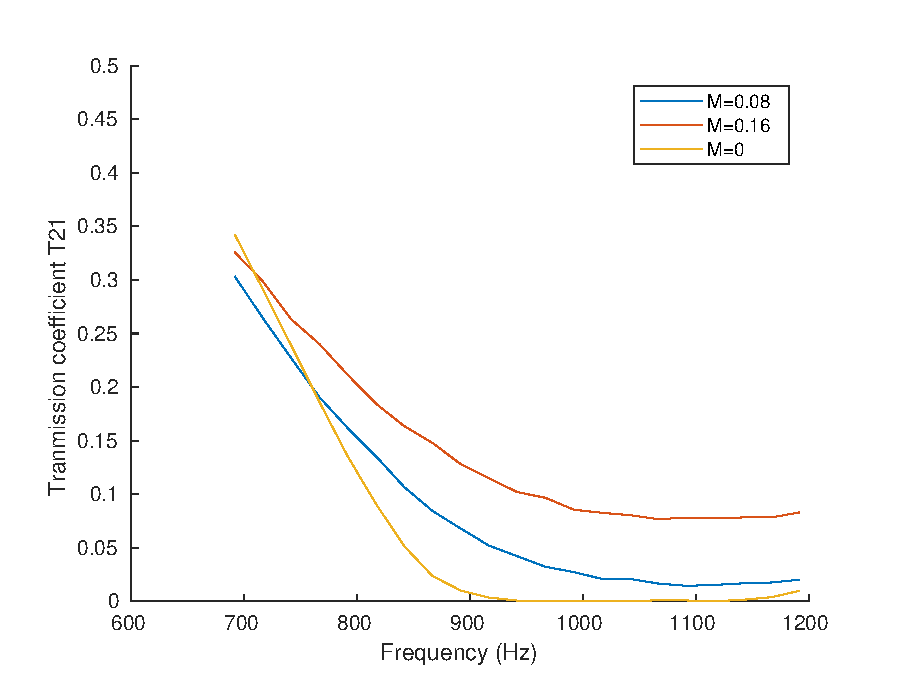
\includegraphics[width=1\linewidth]{T21Lin1}
    \caption{T21}
    \end{subfigure}%
    \begin{subfigure}{.5\textwidth}\centering
     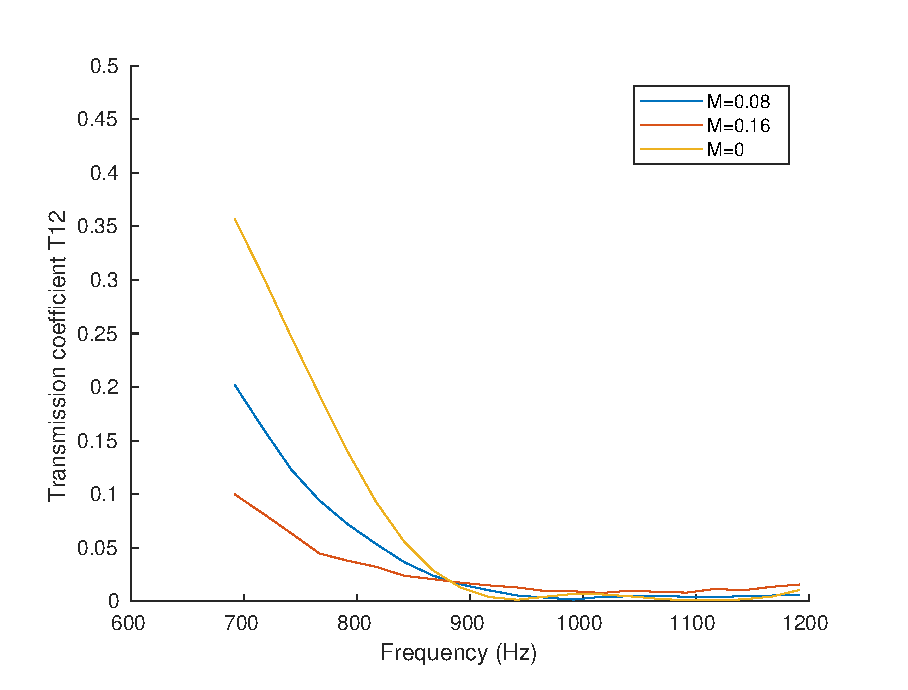
\includegraphics[width=1\linewidth]{T12Lin1}
    \caption{T12}
    \end{subfigure}
    \caption{Transmission coefficients: Liner 1 and M=0, M=0.08, M=0.16}
\end{figure}
Liners should have the same dimensions and the same acoustic properties. However, no-negligible difference between these liners are highlighted:
\begin{figure}[H] \centering
    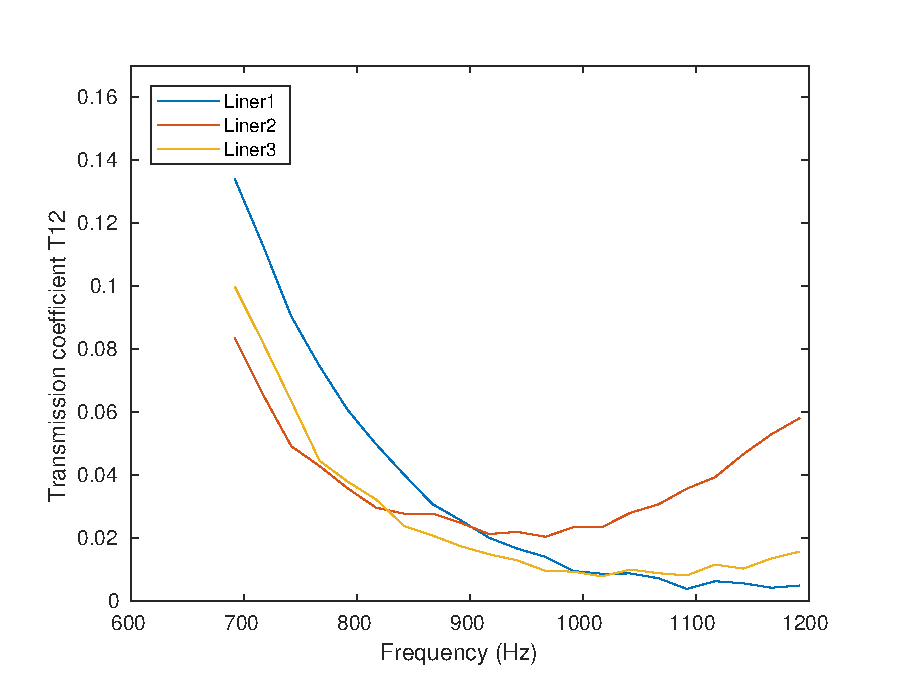
\includegraphics[scale=0.7]{T12M016}
    \caption{Transmission coefficients: liner 1, liner 2, liner 3 for M=0.16 }
\end{figure}
The first results show the expected trends. The setup shows a good repeatability. Indeed two measures with the same liner were done (Two different fixations) and they are very closed.\\
The difference between the liners stays unexplained.
\subsubsection{Acoustic impedance}
A second step of post-treatment is to get the acoustic impedance.

%------------------------------------------------------------------------------------------------------------
%------------------------------------------------------------------------------------------------------------
\clearpage